%%%%%%%%%%%%%%%%%%%%%%%%%%%%%%%%%%%%%%%%%%%%%%%%%%%%%%%%%%%%%%%%%%%%%%%%

%% \CharacterTable
%%  {Upper-case    \A\B\C\D\E\F\G\H\I\J\K\L\M\N\O\P\Q\R\S\T\U\V\W\X\Y\Z
%%   Lower-case    \a\b\c\d\e\f\g\h\i\j\k\l\m\n\o\p\q\r\s\t\u\v\w\x\y\z
%%   Digits        \0\1\2\3\4\5\6\7\8\9
%%   Exclamation   \!     Double quote  \"     Hash (number) \#
%%   Dollar        \$     Percent       \%     Ampersand     \&
%%   Acute accent  \'     Left paren    \(     Right paren   \)
%%   Asterisk      \*     Plus          \+     Comma         \,
%%   Minus         \-     Point         \.     Solidus       \/
%%   Colon         \:     Semicolon     \;     Less than     \<
%%   Equals        \=     Greater than  \>     Question mark \?
%%   Commercial at \@     Left bracket  \[     Backslash     \\
%%   Right bracket \]     Circumflex    \^     Underscore    \_
%%   Grave accent  \`     Left brace    \{     Vertical bar  \|
%%   Right brace   \}     Tilde         \~}

%%%%%%%%%%%%%%%%%%%%%%%%%%%%%%%%%%%%%%%%%%%%%%%%%%%%%%%%%%%%%%%%%%%%%%%

%\documentclass[b5paper,10pt,twoside,cucitura]{toptesi}
\documentclass[b5paper,10pt]{toptesi}

%%%PACKAGES%%%

\usepackage{lipsum}
\usepackage{amssymb} %per i simboli degli insiemi numerici
\usepackage{amsthm} %per \proof e \endproof
\usepackage{ragged2e} %giustifica
\justifying %giustifica
\usepackage{eurosym}
\usepackage{graphicx}
\usepackage{empheq}
\usepackage{xcolor}
\usepackage{amsmath}
\usepackage[T1]{fontenc}
\usepackage[latin1]{inputenc}
\usepackage{lmodern}
\usepackage{hyperref}
\usepackage[titletoc,toc,title]{appendix}

\hypersetup{%
    pdfpagemode={UseOutlines},
    bookmarksopen,
    pdfstartview={FitH},
    colorlinks,
    linkcolor={blue},
    citecolor={red},
    urlcolor={blue}
  }

%%%FRONTISPIECE%%%

\ateneo{Universit{\`a} degli Studi di Milano-Bicocca}
\FacoltaDi{Statistica\\e Metodi Quantitativi per la finanza}
\titolo{Improving Overnight Curve Calibration}
\corsodilaurea{Economia e Finanza}
\candidato{\tabular{@{}l@{}}Nicholas \textsc{Bertocchi}\\matricola: 797940\endtabular}
\relatore{prof.\ Ferdinando Ametrano}
%\secondorelatore{prof.\ .....}
\tutoreaziendale{dott.\ Nicola Moreni}
\NomeTutoreAziendale{Banca IMI}
\sedutadilaurea{\textsc{Anno~accademico} 2015-2016}
\logosede{logo}

\newtheorem{osservazione}{Osservazione} %Standard LaTeX
\begin{document}\errorcontextlines=9 %debugging
\english
\CycleName{cycle}

	\CorsoDiLaureaIn{Master degree course in\space}
	\NomeMonografia{Bachelor Degree Thesis}
	\TesiDiLaurea{Master Degree Thesis}
	\InName{in}
	\CandidateName{Candidate}% or Candidate
	\AdvisorName{Supervisors}% or Supervisor
	\TutorName{Tutor}
	\NomeTutoreAziendale{Internship Tutor:\\Banca IMI}
    \CycleName{cycle}

\frontespizio

%\ringraziamenti

\indici
\mainmatter

%%%ABSTRACT%%%

%\chapter*{Abstract}
%\markboth{\MakeUppercase{Abstract}}{}
%\addcontentsline{toc}{chapter}{Abstract}

%%%INTRODUCTION%%%

\chapter*{Introduction} \label{chap:Intro}
\markboth{\MakeUppercase{Introduction}}{}
\addcontentsline{toc}{chapter}{Introduction}
Every work which seeks to speak about interest rates term structure cannot avoid to begin from 2007 liquidity and credit crisis. Before that harmful year every market participants considered the credit risk on short time frame, for example less then one year, irrelevant and this opinion was reflected by the market in infinitesimal basis spread between different tenor rates. In other words, all banks in the system consider almost the same lend money to other banks for a year, for a month or for a day. This context was possible because a big financial institution's default probability was seen as negligible but, otherwise, it wasn't, as the Lehman Brothers case teach to the world. The panic in the markets during summer 2007 drives first to a crisis of confidence between the so called "Too big to fail" \footnote{This title was created during subprime crisis to speak about financial institutions that, as the nickname suggest, are so big that their default might means the overall system collapse} that, unable to estimate other institutions creditworthiness, can't no more trust each other and this leads to a situation in which it was preferable to be paid with higher frequency in order to mitigate counterparts credit risk. The direct consequence was that Libor as well as Euribor rates with different tenors shown different portions of credit/liquidity spread which became higher as tenor increase. That was the end of the Single-Curve World. The basis explosion is shown in Figure \ref{fig:basisafter} and it is important to underlying that this effect was not due to a correlation break, as the Figure \ref{fig:correlationbreak} suggest. From that time every implied relationship between interest rates failed and it become necessary to calibrate, for each currency, multiple forwarding curve and particular relevance was given to the Overnight Curve which plays the role of forwarding curve for its specific tenor and the role of exogenous discounting curve for each tenor. This double function is due to the fact that all interest rate derivatives traded on regulated markets (like Futures) or collateralized with daily margining (like Forward Rate Agreements, Swaps and Basis Swaps) settle their positions on collateral accounts which earn the overnight rate and this is why the overnight curve usually plays the role of discounting curve as well as the role of forwarding curve.\\

\begin{figure}[!h]
\centering
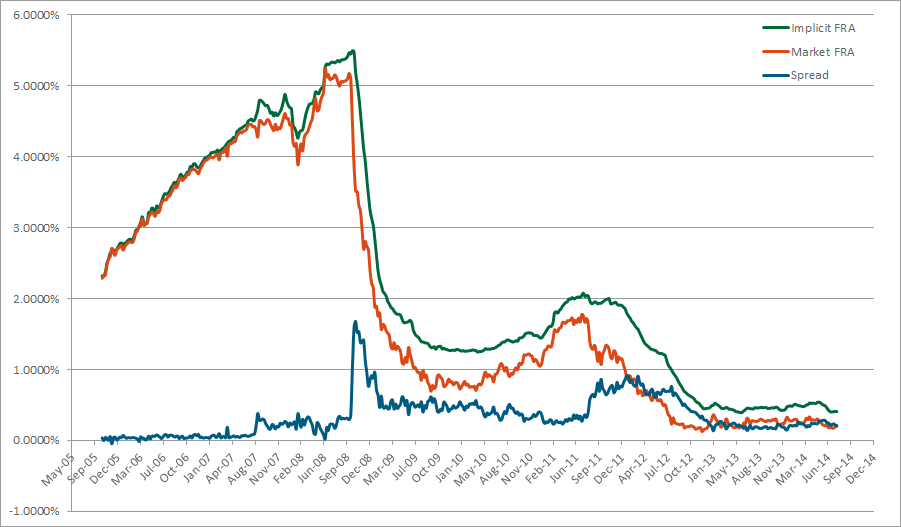
\includegraphics[width=0.8\textwidth]{images/basisafter}
\caption{After summer 2007 the $3X6$ FRA implicit in Euribor 6M and Euribor 3M fixings it was no longer consistent with the $3X6$ FRA quoted by the market.}
\label{fig:basisafter}
\end{figure}
        
\begin{figure}[!h]
\centering
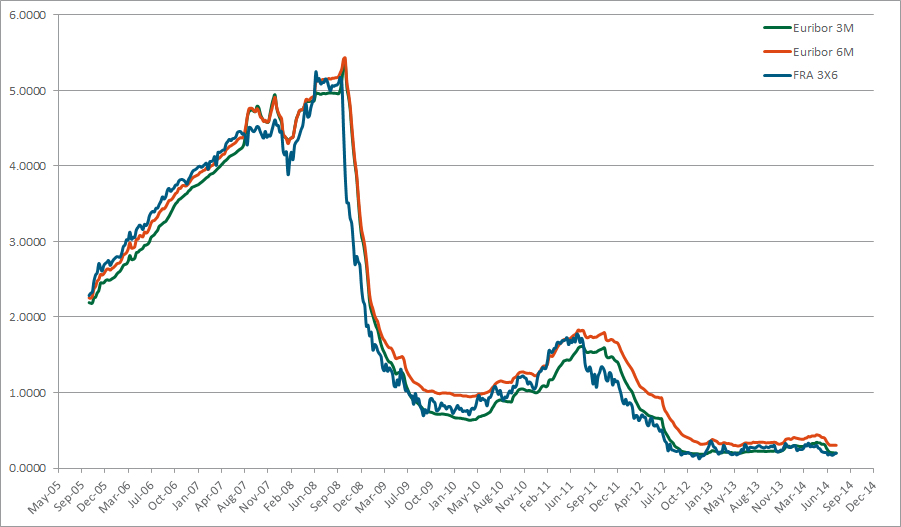
\includegraphics[width=0.8\textwidth]{images/correlationbreak}
\caption{The effect shown in previous figure can not be attributed to a correlation break.}
\label{fig:correlationbreak}
\end{figure}

\newpage
This work aims to discuss how a "state of art" overnight curve can be calibrated starting from some general rate curve bootstrapping issues, presented in Chapter \ref{chap:1}, like:

\begin{description}
    \item{-} Curve parametrization;
    \item{-} Bootstrap Algorithms;
    \item{-} Pillar interpolation technique.
\end{description}
After that, Chapter \ref{chap:2} will be focused on the overnight curve construction explaining which kind of choice are preferable passing through the same points outlined in Chapter \ref{chap:1}.
Finally, Chapter \ref{chap:3} represents the core of this work and analyze some peculiar overnight problems outlining different solutions in order to improve the curve quality. In particular this points will be stressed:

\begin{description}
    \item{-} A Mixed Interpolation technique to respect empirical evidence;
    \item{-} Forward Stub utilization to prevent overlapping instruments;
    \item{-} Jumps and Turn of Year \textit{(TOY)} effect in foreign currencies curves (the GBP and USD problem will be presented);
    \item{-} Fed Funds Arithmetic Average Coupon OIS introduction to Increase USD curve smoothness.
\end{description}

%%%CHAPTER1%%%

\chapter{Rate Curve Bootstrap} \label{chap:1}
This first chapter wants to outline the most important issues concerning rate curves calibration in a general point of view. Every argument discussed here can be applied to all rate curves and is not specific of the Overnight case which, instead, will be discussed in the next chapter.

    \section{Parametrization} \label{section:1.1}
    Choosing the rate curve parametrization means decide how the curve must be described. There are three workable solution that can be adopted, namely:\\
    
    \begin{description}
        \item{-} Description through Instantaneous Forward Rates ($f\ped{inst}$)
        \item{-} Description through Zero Rates ($z(t\ped{1})$)
        \item{-} Description through Pseudo-Discount Factors ($P(t\ped{1}$)) \footnote{For a more detailed description of Forward Rates, Zero Rates and Discount Factors see \ref{app:typesofrates}}\\
    \end{description}

    Since this relationship is true:
    
    $$P(t\ped{i}) = e^{-z(t\ped{i})t\ped{i}} = e^{\int_{0}^{t\ped{i}} f\ped{inst} ds}$$
    \\
    or equivalently:
    
    $$-\ln(P(t\ped{i})) = -z(t\ped{i})t\ped{i} = \int_{0}^{t\ped{i}} f\ped{inst} ds$$
    \\
    the three solutions are almost equal except for the Pseudo-Discount Factors case which is the only one well defined for $t=0$ (where the value is $1.00$)\footnote{In the following sections will be shown that this is one of the reason why the pseudo-discount factor parametrization is the most often used}
    
        \subsection{Possible Description through Forward Rates} \label{subsection:1.1.1}
        Each rate curve $C_{x}$ is a forwarding curve linked to a specific tenor $x$. The most natural parametrization should be the one that models directly forward rates because the market quotes forward rates (and not other quantities like discount factors). Forward rates directly quoted by the market through FRA, Futures and indirectly through Interest Rates Swaps and Basis Swaps, are simple forward rates corresponding to a triplet $(s,s+x,\tau_{x})$ where $s\geq t$ and $\tau_{x}$ is the specific day count convention related to the underlying index of each instrument (example: Euribor $xM$). So our curve $C_{x}$ should be described by:
        $$C_{x}(t)=\{s\rightarrow F_{x}(t;s,s+x)|s\geq t\}$$
        Unfortunately, this is not the commonly used approach.
        
        \subsection{Classical solution through Pseudo-Discount Factors}  \label{subsection:1.1.2}
        As a consequence of the relationship between $P(t\ped{1})$, $z(t\ped{1})$ and $f\ped{inst}$ it is always possible to derive a forward rate via pseudo-discount factor by means of the following equation:
        
        $$F_{x}(t;s_{1},s_{2})=\frac{1}{\tau(s_{1},s_{2})}\left(\frac{P_{x}(t;s_{1})}{P_{x}(t;s_{2})}-1\right)$$\\
        
        In the old Single-Curve World this relationship was a result of a no-arbitrage condition which does not hold anymore but now, in a Multi-Curve System, this is merely the definition of a {\it pseudo-discount factors} function $P_{x}(t;s)$.\\
        To clarify this concept let's make the following example. In the old Single-Curve world, before 2007 crisis, in the EUR market it was possible to could calculate the forward rate $F(t;t+3M,t+6M)$ starting from the values $P(t;t+3M)$ and $P(t;t+6M)$ deduced from Euribor $3M$ and Euribor $6M$ fixings with a no arbitrage condition; the resulting value was in line with the market quote of the $3X6$ FRA. With the large Basis Swap spreads presently quoted on the market this relation is no more valid: if we calculate the $3X6$ FRA implicit in Euribor 6M and Euribor 3M fixings (as explained above) we do not obtain the $3X6$ FRA quoted by the market (see Figure \ref{fig:basisafter}).
        The discussion above has proved that for each forward curve $C_{x}$ exist three alternative descriptions :
        
        $$C_{x}(t)=\{s\rightarrow P_{x}(t;s)|s\geq t\}$$
        $$C_{x}(t)=\{s\rightarrow z_{x}(t;s)|s> t\}$$
        $$C_{x}(t)=\{s\rightarrow f_{x}(t;s)|s> t\}$$
        
        The advantage of the pseudo-discount factor description (compared to a direct forward rates description) is that, as already mentioned, they are well defined for $t=0$. On the other hand the drawbacks are obvious. First of all, it implies to not model directly the market quantities. Secondly the function $P_{x}(t,s)$ has an arbitrary part of length $x$ that must be chosen. When $x=ON$ this arbitrary part is really small (few days) and it can be fixed with some market quotes. So in this case we can use the pseudo-discount factors description without problems at all and is also consistent with the role of $C_{ON}$ as discount curve of the framework (in this case pseudo-discount factors are real discount factors!). For the other tenors it is necessary to introduce synthetic deposits in order to manage this arbitrariness. However, the description of synthetic deposits is outside this work's objectives.
        
    \section{Calibration Algorithms} \label{section:1.2}
    Pricing of all interest rate derivatives requires modelling the future dynamics of the zero rates (or yield) curve term structure. A key point to understand is that finding the best way to build the rates term structure is crucial in order to obtain reasonable prices, since an incorrect one will fail to produce them. The aim to which we have to be targeted on when calibrating an yield curve is to minimize, or eliminated, repricing errors especially on the most liquid instruments that are the one preferred for calibration as it will be discussed in \ref{section:2.1}.
    In order to fulfil our task of error minimization there are different ways that can be divided into 2 main classes that, as a common condition, both require a set of $N$ pre-selected market instruments:
    \begin{itemize}
        \item Best-Fit Algorithm
        \item Exact-Fit Algorithm
    \end{itemize}
       
        \subsection{Best-Fit Algorithm} \label{subsection:1.2.1}
        A {\it best-fit algorithm} assumes a functional form for the curve $\{C_{x}\}$ and calibrates its parameters using the pre-selected instruments. It is very popular due to the smoothness of the output curve, calibration easiness and intuitive financial interpretation but it has a big drawback: usually there are more instruments than parameters and this lead to a relevant problem consisting in an imperfect reprice of the whole set of instruments. The merely fact that a best-fit calibration minimize instead of eliminate repricing errors means that this kind of algorithm are not good enough for trading purposes in liquid markets, where the Bid/Ask spread closeness implies that a basis point quarter can make the difference.
        
        \subsection{Exact-Fit Algorithm} \label{subsection:1.2.2}
        {\it Exact-fit algorithms}, instead, fix the yield curve on a time grid of $N$ points (or {\it pillars}) in order to exactly reprice the selected instruments. To do that, An interpolation method is required to determine curve values between pillars. Usually the algorithm is incremental, building the curve step-by-step with the increasing maturity of the ordered instruments ({\it bootstrap} approach).\\
        The set of bootstrapping instruments defines the time grid used for bootstrapping: each pillar is the maturity date or the last relevant date of the corresponding instrument.
        The interpolation method is strictly connected to the bootstrap and plays a fundamental role also during bootstrapping and not just after that. The "pillar-to-pillar" calibration proceeds with incomplete information; so, in order to determine each pillar value, the already bootstrapped part of the curve has to be used and, in particular, both pillar and intermediate interpolated values. This is the reason why we need to interpolate during the bootstrap algorithm and it also explain why this process is iterative. In fact, if the algorithm determines next pillar value taking advantage of the pre-bootstrapped part of the curve, it is straightforward that this value is influenced by it. Since including a pillar means add new information concerning the curve dynamic, if a {\it global interpolation scheme} is used, this tends to alter the first curve part shape (as it will be discussed in \ref{subsection:1.3.1}). This is usually remedied by cycling in iterative fashion: after a first bootstrap the resulting complete grid is altered one pillar at time using again the same bootstrapping algorithm, until convergence is reached (see \cite{haganwest} for a practical example of this interaction between interpolation and bootstrap).\\
        Clearly, this kind of algorithms are more accurate; henceforward the analysis will be restricted to the exact curve calibration problem.
   
    \section{Interpolation Techniques} \label{section:1.3}
    Whatever parametrization and algorithm has been chosen, an interpolation for off-grid dates/times is needed. An interpolation technique always work with two distinct objects:
    \begin{description}
        \item{-} the quantity to be interpolated;
        \item{-} the interpolation scheme.
    \end{description}
    The quantity to be interpolated is chosen according to curve's description. If a forward rates description is used, the most reasonable quantity to be interpolated is the forward rate itself: in this way interpolation schemes and constraints can be imposed directly on market quantities. If, instead, a pseudo-discount factors description is used (and this is our case as it will be discussed in \ref{subsection:1.3.1}), the following main choices can be chosen:
    
     \begin{itemize}
         \item Discount factors;
         \item Zero rates;
         \item Instantaneous forward rates.
     \end{itemize}
   In particular discount factors have exponential decay and this characteristic can leads to excess of convexity; so it makes sense to interpolate on log-discounts to ensure a smoother decay. Before analyzing the different impact of different choices on curve smoothness it is necessary to introduce the interpolation scheme concept. 
        
        \subsection{Local scheme Vs. Global scheme} \label{subsection:1.3.1}
        All interpolation techniques can be grouped together into two different classes:\\
        \begin{itemize}
        \item{\bfseries Local scheme}: With a local scheme each intermediate point depends only on its bracketing pillars. Notice that when bootstrapping with a local interpolation the curve's shape between two calibrated pillars can no longer change. This kind of scheme use only $\{y\ped{i}\}$ near $\{t\ped{i}\}$ to calculate each $\{y'\ped{i}\}$ and a typical example is the linear interpolation.
        \item{\bfseries Global scheme}: Conversely, with global scheme, each intermediate point depends on points outside the interval defined by its neighborhoods pillars. If the interpolation method is global, the curve changes continuously until the end of the procedure because the shape of already bootstrapped part of the curve is altered by the addition of further pillars. Cubic spline are the most common examples of global interpolations that are fully defined when function values $\{y\ped{i}\}$ at point $\{t\ped{i}\}$ are supplemented with function first derivatives values $\{y'\ped{i}\}$.
        \end{itemize}
        
        \begin{figure}[!h]
        \centering
        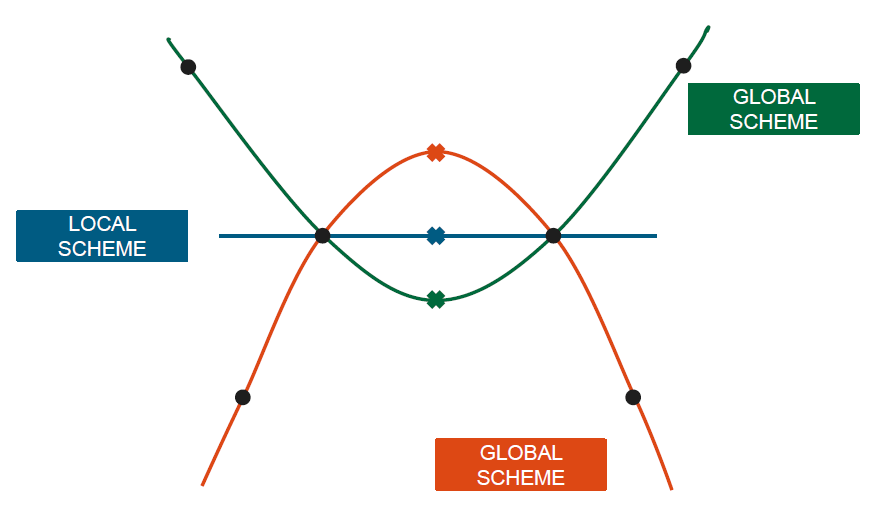
\includegraphics[width=0.7\textwidth]{images/scheme.PNG}
        \caption{Local scheme Vs. Global scheme interpolation.}
        \label{fig:scheme}
        \end{figure}
        
        The criteria used to analyse the interpolation techniques usually fall into one of the following two categories:
        
        \begin{itemize}
        \item the quality of the forward rates: in this case the output curve is an "accounting" tool that wants to produce smooth forward rates; 
        \item the quality of the implied hedging strategies: in this case the output curve is a "risk management" tool that tries to produce reasonable and stable implied hedging quantities.
        \end{itemize}
        Sometimes an interpolation method is good to build forward rates but not good from an hedging point of view (This is the case of cubic spline). Since the implementation of hedging curve is not a target of this thesis, the analysis will be restricted on building high quality forward rates and so the best interpolation technique will be the one which is able to produce the best forward rates in terms of smoothness. The most popular interpolation techniques are:
        
        \begin{description}
            \item{-} Linear interpolation on zero rates or discount factors;
            \item{-} Linear interpolation on log-discounts;
            \item{-} Constrained cubic spline interpolation on zero rater or log-discounts;
            \item{-} Monotonic cubic natural spline interpolation on zero rates or log-discounts;
            \item{-} Mixed interpolation.
        \end{description}
        The description of the this interpolation techniques is postponed to Section \ref{section:3.1} where it will be also introduced the Mixed Interpolation which it is assumed to be the best way to interpolate the overnight curve;
        
%\blankpagestyle{headings}
%\lipsum[1-2]

%%%CHAPTER2%%%

\chapter{Overnight Curve Definition} \label{chap:2}
This chapter wants to focus on overnight curve construction passing through every issue outlined in Chapter \ref{chap:1}. The objective is to present a calibration best practice related on the specific overnight curve case which is the core argument of this work.

    \section{Instrument selection criteria} \label{section:2.1}
    Before 2007, in the Single-Curve World, fixed income pricing requires to model just one curve named the Standard Curve. This particular curve was calibrated selecting among a wide range of instruments with different tenors. Market instruments were more than needed and this permits to calibrate a curve with a high pillar density in which the only problem was to choose the best set of instruments following a liquidity criteria. \\
    The liquidity criteria implies that the major selection priority is given to the most liquid instruments available on the market. This principle is followed because instrument's liquidity is due to the trade volume. The more an instrument is traded and the more his value tends to be fair because of market efficiency. The bootstrap algorithm must be fed only with fair quotes, which vehicle the most efficient information, in order to calibrate a fair curve. It is strictly not recommended to bootstrap illiquid quotes in order to bootstrap market efficient information instead of market noise. \\
    Since the beginning of the Multi-Curve World, the curve selection criteria become more difficult due to the fact that every curve has to be built using his specific tenor instruments. In addiction many interest rate derivatives have become illiquid and the wide range of market quotes has decreased dramatically. The present multi-curves have a far less pillar density compared to the old standard one (this is the reason why synthetic deposits are necessary) and this limits the outcome quality. Fortunately, in the overnight case, there are many liquid instruments that can be used to cover all the curve behaviour, from the short term to the last section (usually from spot date to 60 years). In particular overnight curve is bootstrapped using the following instruments:
    
    \begin{itemize}
    \item ON and TN Deposits in order to set the curve reference date to today's date (these instruments are not properly based on Eonia - the underlying index is the one-day tenor Euribor - thus we are introducing a very small inconsistency);
    \item all the available forward starting OIS on ECB dates;
    \item spot starting OIS up to 60Y.
    \end{itemize}
    
    The ECB OIS are more liquid than spot starting OIS and this is way they are always used when available. However, introducing forward start ECB OIS leads to a overlapping instruments problem that can be fixed using a forward Stub, as it will be discussed in \ref{section:3.2}. Next section will describe in detail this kind of instruments.
    
        \subsection{Overnight Deposits} \label{subsection:2.1.1}
        \textit{Interbank Deposits} are unsecured loans made by a bank to another bank. \textit{Deposits} are standard money market zero coupon contracts, where the \textit{Lender} pays at start day (\textit{settlement day}) a notional amount $N$ to the \textit{Borrower} and he receives back the notional amount $N$ plus the interest earned over the period that goes from settlement date to maturity date. The \textit{Deposits} description have to take care of $3$ important dates:
        
        \begin{itemize}
        \item \textit{Fixing date} ($t_{0}^F$) or today: the date in which we fix the interest rate that will be applied on our \textit{Deposit};
        \item \textit{Settlement Date} or \textit{Spot Date} ($t_{0}$): the date in which our \textit{Deposit} starts to accrue interest;
        \item \textit{Maturity Date} ($t_{1}$): the date in which the contract ends and the notional plus the interests earned are paid back.
        \end{itemize}

        The interest rate applied is annual and it is simply compounded; it is called \textit{Deposit rate} and we denote it as $r_{t}^{Depo}$. The payoff of this contract at maturity date ($t_{1}$) is:
     
        $$Depo_{t_{1}}(t_{1}) = N \cdot (1 + r_{t_{1}}^{Depo}\tau_{0,1})$$ 
     
        Where: $\tau_{0,1}$ is the \textit{year-fraction} between $t_{0}$ and $t_{1}$.

        To compute the present value ($t_{0}^F$) of this \textit{Deposit} it is necessary to discount his unique cashflow:
     
        $$Depo_{t_{1}}(t_{0}^F) = D(t_{0}^F,t_{1})\cdot Depo_{t_{1}}(t_{1}) = N$$
     
        and since: 
        
        $$r_{t_{1}}^{Depo} = r_t \mbox{(the Zero-Rate)}$$
        
        the discount factor is: 
        
        $$D(t_{0}^F,t_{1}) = \frac{1}{(1+r_{t_{1}}^{Depo}\tau_{0,1})}$$.\\

        These contracts are quoted and exchanged on the \textit{Interbank OTC (Over The Counter) market} for various currencies and maturities, that usually do not go beyond the year. However the first 2 maturities are a bit different from the others: 
        
        \begin{itemize}
        \item \textit{OverNight (ON)}: it is a \textit{Deposit} that starts today, at \textit{Fixing Date} ($t_{0}^F$), lasts for one day, and ends tomorrow ($t_{0}^F$+1);
        \item \textit{Tomorrow-Next (TN)}: this contract starts tomorrow ($t_{0}^F$+1), lasts for one day, and ends the day after tomorrow ($t_{0}^F$+2); for example in EURO market, where settlement date is today plus 2 business days, this contract starts tomorrow (the next business day after today) and ends at settlement date.
        \end{itemize}
        
        After ON and TN \textit{Deposit}, there is the  \textit{Spot-Next (SN)} that is a regular contract: starts at \textit{Spot Date}, or settlement date ($t_{0}$), lasts for one day, and ends the day after ($t_{0}+1$). The following \textit{Deposits} are denoted with their maturity, e.g.  $SW$ (Spot Week), $1M$ (1 Month), $3M$ (3 Months) and so on. The \textit{Business Day Convention} is \textit{Following} for maturities shorter then 1 month and \textit{Modified Following} for longer maturities.
        
        \subsection{Interest Rate Swap {\it (IRS)}} \label{subsection:2.1.2}
        Interest Rate Swaps (IRS) are OTC contracts in which two counter-parties agree to exchange two streams of cashflows typically tied to a floating LIBOR or EURIBOR rate, $L(t_{i-1},t_{i})$, versus a fixed rate $r^{IRS}$. IRS can be seen as a set of consecutive FRAs; on a number of future dates a fixed interest rate, $r^{IRS}$, will be exchanged for a floating interest rate (LIBOR). The payments dates of the floating rate and the fixed rate can be different, in that case it is still possible to see IRS as a portfolio of FRAs, part of them with a null fixed or floating rate (those with single-direction payment). All payments are based on the same notional $N$ and are settled at the end of each period. \\
        An IRS is characterized by two schedule of payments, one for the floating rate, the so called \textit{floating leg}, and one for the fixed rate, the \textit{fixed leg}:
        
        \begin{itemize}
        \item \textit{floating leg dates} = $\{t_0,t_1, ... , t_n\}$;
        \item \textit{fixed leg dates} = $\{s_0,s_1, ... , s_m\}$;
        \end{itemize}
        
        with: $t_0 = s_0$ and $t_n = s_m$;\\
        
        The coupon payoffs in one time interval, between $t_i$ and $t_{i-1}$ for the floating leg and between $s_j$ and $s_{j-1}$ for the fixed leg, evaluated at the end date of the period, are (with notation $IRS_{leg}$($evaluation$-$date$; $start$-$date$, $end$-$date$, $rate$)):
        
        \begin{align}
        &IRS_{float}(t_i;t_{i-1},t_i,L) = N \cdot L(t_{i-1},t_i) \cdot \tau_{i-1,i} \\ 
        &IRS_{fixed}(s_j;s_{j-1},s_j,r^{IRS}) = N \cdot r^{IRS} \cdot \tau_{j-1,j};
        \end{align}

        The fixed interest rate of the contract, $r^{IRS}$, is calculated such that the $NPV$ of the contract at $t_0$ is equal to $0$, so:

        $$NPV(t_0) = \sum_{i=1}^n IRS_{float}(t_{i-1};t_{i},t_i,L(t_i,t_{i-1}))\cdot D(t_0,t_i)$$\\
        $$- \sum_{j=1}^m IRS_{fixed}(s_j;s_{j-1},s_j,r^{IRS}) \cdot D(s_0,s_j) = 0$$

        Solving for $r^{IRS}$ we can find the correct rate, called \textit{Swap fair rate}.
        
        $$r^{IRS} = \frac{\sum_{i=1}^n (L(t_{i-1},t_i) \cdot \tau_{i-1,i}\cdot D(t_0,t_i))}{\sum_{j=1}^m (\tau_{j-1,j} \cdot D(s_0,s_j))}$$\\
        
        A particular case of IRS are Overnight Indexed Swap (OIS) where the floating leg is tied to the overnight rate. Payments of the floating leg are not done every day, but at specific coupon dates, the fixed leg dates, and therefore the floating rate is daily compounded over that period. The fixed rate for $OIS$ is normally a simple rate with interest at maturity date, for $OIS$ shorter than 1 year, and it is an annual rate for longer maturities. \\
        The floating leg is:
        
        $$IRS^{OIS}_{float}(t_i;t_{i-1},t_i,R^{ON}(t_{i-1},t_i)) = N \cdot R^{ON}(t_{i-1},t_i) \cdot \tau^{ON}_{i-1,i}$$ 

        Since $R^{ON}(t_{i-1},t_i)$ is daily compounded, with $M$ indicating the number of business days between $t_{i-1}$ and $t_{i}$, we have ($t_{{i-1}_{0}}=t_{i-1}$, $t_{{i-1}_{M}}=t_{i}$):

        $$1+R^{ON}(t_{i-1},t_i) \cdot \tau^{ON}_{i-1,i} = \prod_{k=1}^M (1 + r^{ON}(t_{{i-1}_{k-1}},t_{{i-1}_k})\tau^{ON}_{{i-1}_{k-1},{i-1}_{k}})$$
        $$R^{ON}(t_{i-1},t_i) = \frac{1}{\tau^{ON}_{i-1,i}} \cdot \left(\prod_{k=1}^n (1 + r^{ON}(t_{{i-1}_{k-1}},t_{{i-1}_k})\tau^{ON}_{{i-1}_{k-1},{i-1}_{k}}) - 1\right)$$\\

        For determine the $r^{OIS}$ rate we proceed like a simple IRS contract. We calculate the $NPV$ of the swap and we impose that his value in $t_0$ is equal to 0. Since overnight rate is now regarded as a better proxy for the risk-free rate than the LIBOR, it can be used even for discounting; therefore:

        $$\sum_{i=1}^n (R^{ON}(t_{i-1},t_i) \cdot \tau^{ON}_{i-1,i}\cdot D(t_0,t_i)) = \sum_{i=1}^n (D(t_0,t_{i-1}) - D(t_0,t_i))$$\\
        $$= 1 - D(t_0,t_n)$$

        This is the so called telescopic property of floating leg of the $OIS$. Using this result:
        
        $$r^{OIS} = \frac{1 - D(t_0,t_n)}{\sum_{i=1}^n (\tau^{ON}_{i-1,i} \cdot D(t_0,t_i))}$$\\
        
        Which is the OIS rate. \\
        
    \section{Calibration choices} \label{section:2.2} 
    The construction of the $ON$-curve follows the old single curve approach. The only real difference is the selection of the instruments: as sad before, it is necessary to choose \textit{homogeneous} quoted products, based on the same underlying rate (\textit{Eonia} in this case); namely:
    
    \begin{itemize}
    \item ON,TN,SN Deposits
    \item forward EONIA OIS on ECB dates, up to 6M; they cover the time interval between two consecutive ECB Meeting dates;
    \item OIS on EONIA from short maturity (SW,2W,..) up to 30Y, 50Y, 60Y, depending on the available quotations.
    \end{itemize}

    Note that the first three instruments are based on Euribor 1D tenor and not on EONIA; doing this, a little inconsistency is introduced. Otherwise, these deposits are useful to cover the very short term of the curve. An important property of $ON$ rates is that they are relatively constant between the Monetary Policy Meeting Dates relevant to each currency, (see \cite{ECB}); these meetings fix the short-term accommodation policy rates and overnight interest rates follow the direction of this policy. Forward $OIS$ on ECB Dates reflect these market expectations and it is very important to use them for building the first section of the curve. \\
    The construction of the overnight curve can be divided into at least 2 section, where different approaches should be:
    
    \begin{itemize}
    \item \textit{Short Dated Region}: in this region the effect of expected rate change on Meeting Dates predominates; that's why, here, empirical evidence shows a piece-wise constant curve, with possible jump behavior in rates around Meeting Dates. Rates can also show this behavior in other dates, typically at month, quarter and year ends or on dates where there are large structural flows. This behavior must be treated carefully to avoid errors and will be treated in \ref{section:3.3}.
    \item \textit{Long Dated Region}: in this section the curve show the typical smooth behavior and so, the standard bootstrapping process can be used.
    \end{itemize}
    
    This particular overnight behaviour (piece-wise constant in short region and smooth in long region) can be fixed using two different kinds of interpolations: linear on log discount and monotonic cubic natural spline on log discount \footnote{the characteristic of this mixed interpolation will be treated in \ref{section:3.1}.}. The linear one is tipically used for pricing purpose in the short term section of the curve (for example to obtain the quotation of $OIS$ up to 1-2 years) and the cubic one for discounting or long term pricing. \\
    Figure 
    
    \begin{figure}[!h]
    \centering
    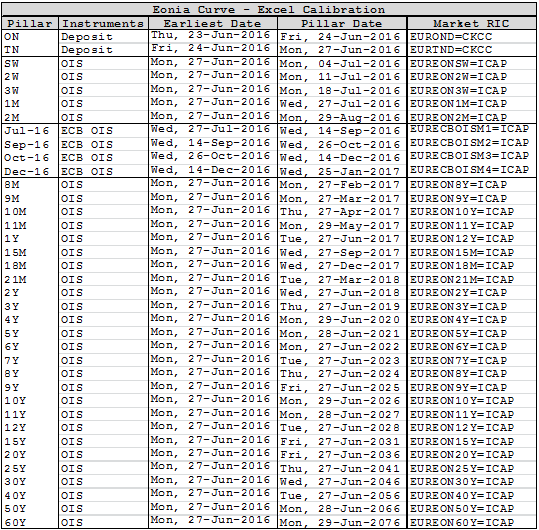
\includegraphics[width=0.9\textwidth]{images/ONcurve.png}
    \caption{An example of overnight curve instrument selection which respects the criteria previously discussed.}
    \label{fig:ONcurve}
    \end{figure}
    
%\selectlanguage{english}
%\EnableFigTabNames

%%%CHAPTER3%%%

\chapter{Improving Overnight Curve} \label{chap:3}
    \section{Defining the Best Interpolation Method}\label{section:3.1}
    All requirements to present some of the most popular interpolation techniques (i.e. quantity to be interpolated plus an interpolation scheme) have been already discussed in Section \ref{section:1.3}; let's introduce them stressing on every pros and cons.\\
    Since each simple forward rate is approximately the integral of instantaneous forward rates, the smoothness of simple forward rates will be analyzed computing instantaneous forward rates. The starting point is a set of known curve's points $\left\{ (t_{i},y_{i}=y(t_{i}))\right\}_{i=1,...,N}$ where $y$ represent the quantity to be interpolated as defined above. $t_{0}$ will be the reference date.
        
        \subsection{Linear and Log-Linear interpolation} \label{subsection:3.1.1}
        This is a poor and simple way to interpolate that can be computed directly on zero rates (Linear) or on log-discounts (log-linear). For $t \in [t_{i-1}, t_{i}]$ the piecewise linear interpolation formula for zero rates is:\\
        
        $$z(t)t=\frac{t-t_{i-1}}{t_{i}-t_{i-1}}z(t_{i})t+\frac{t_{i}-t}{t_{i}-t_{i-1}}z(t_{i-1})t$$\\
        This kind of interpolation techniques produces the so called: "Sawtooth forward rates" as visible in Figure \ref{fig:sawtooth} and \ref{fig:piecewiselinear}: \\
        
        \begin{figure}[!h]
        \centering
        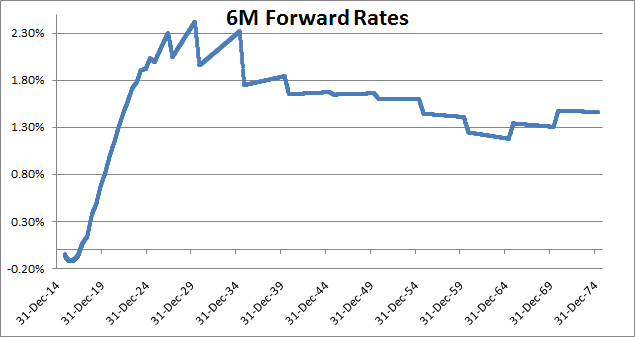
\includegraphics[width=0.7\textwidth]{images/sawtooth.png}
        \caption{An example of sawtooth curve obtained through linear interpolation on zero rates.}
        \label{fig:sawtooth}
        \end{figure}
        
        \begin{figure}[!h]
        \centering
        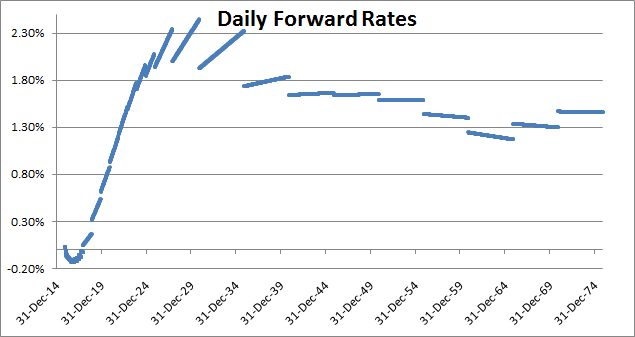
\includegraphics[width=0.7\textwidth]{images/piecewiselinear.png}
        \caption{Forward rates obtained through piecewise linear interpolation on zero rates.}
        \label{fig:piecewiselinear}
        \end{figure}
        
        \newpage
        Obviously, this is not a good way to interpolate quantitites; forward rates are far to be smooth and curve shape is quite improbable.
        In the log-discount case, instead, the interpolation formula becomes:\\
        \\
        $$z(t)t=-\ln P(t)=-\frac{t-t_{i-1}}{t_{i}-t_{i-1}}\ln P(t_{i})-\frac{t_{i}-t}{t_{i}-t_{i-1}}\ln P(t_{i-1})$$\\
        \\
        In this case the output is the so called: "Stepped curve" as visible in Figure \ref{fig:stepped} and Figure \ref{fig:piecewiseflat}. 
        
        \begin{figure}[!h]
        \centering
        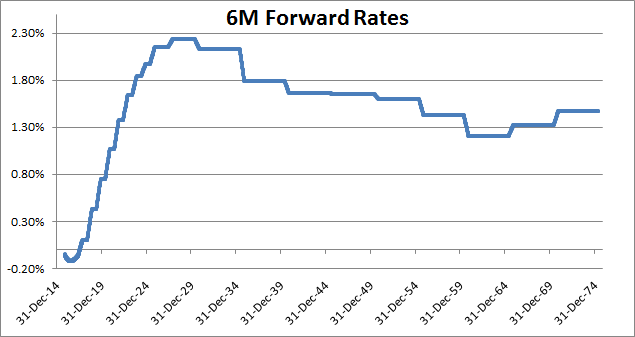
\includegraphics[width=0.7\textwidth]{images/stepped.png}
        \caption{An example of stepped forward rates obtained through linear interpolation on log-discounts.}
        \label{fig:stepped}
        \end{figure}
        
        \begin{figure}[!h]
        \centering
        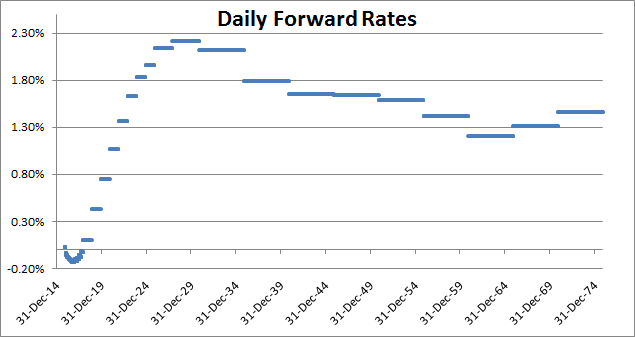
\includegraphics[width=0.7\textwidth]{images/piecewiseflat.png}
        \caption{Piecewise flat forward rates obtained through linear interpolation on log-discounts.}
        \label{fig:piecewiseflat}
        \end{figure}
        
        \newpage
        The result is not better than the one obtained with the linear interpolation on zero rates. Nevertheless this method is more popular because it can be used to describe the first section of overnight-related curves; In fact, market evidence shows that short rates tend to be constant (flat) between particular dates, namely the ones in which there is a European Central Bank monetary policy board meeting. Therefore, the overnight curve is a particular case in which smoothness is a requirement not strictly recommended before the last ECB meeting date published (usually maximum 1 year and a half forward) but returns to be important after it. In this situation using a piecewise flat interpolation or a cubic one for the whole curve might be not accurate in both cases and so a merger of both interpolation techniques is needed which leads to the so called: "Mixed interpolation" that will be treated in \ref{subsection:3.1.4}. \\
        
        \subsection{Constrained Cubic Spline interpolation: The Kruger Scheme} \label{subsection:3.1.2}
        Traditional cubic spline interpolation methods describe the unknown function $f$ as a collection of $N-1$ spline functions $f_{i}$ ($i=1,...,N-1$), each one defined on the interval $[t_{i},t_{i+1}]$ through the following criteria:
        \begin{itemize}
        \item $f_{i}$ is a third order polynomial
        $$f_{i}(t)=a_{i}+b_{i}t+c_{i}t^{2}+d_{i}t^{3}$$
        for $i=1,...,N-1$
        \item $f_{i}$ pass through all the known points
        $$f_{i}(t_{i})=y_{i}\text{ , }f_{i}(t_{i+1})=y_{i+1}$$
        for $i=1,...,N-1$
        \item First order derivative is the same for both functions on either side of a point 
        $$f^{\prime}_{i}(t_{i+1})=f^{\prime}_{i+1}(t_{i+1})$$
        for $i=1,...,N-2$
        \item Second order derivative is the same for both functions on either side of a point
        $$f^{\prime\prime}_{i}(t_{i+1})=f^{\prime\prime}_{i+1}(t_{i+1})$$
        for $i=1,...,N-2$
        \end{itemize}
        The first equation give us $4N-4$ unknown parameters; the other equations give us $2(N-1)+(N-2)+(N-2)=4N-6$ equations. The two remaining equations are based on a border conditions for the starting and ending points. If we choose the following conditions:
        $$f^{\prime\prime}_{1}(t_{1})=f^{\prime\prime}_{N-1}(t_{N})=0$$
        the resulting spline is called {\it Natural Spline}. These interpolation methods suffer of well-documented problems, such as spurious inflection points, excessive convexity, lack of locality and wide oscillations (the spline only alleviates the problem of oscillation seen when fitting a single polynomial). \\
        The Kruger's method (see \cite{kruger}), which combines the smooth curve characteristics of spline interpolation with non-overshooting behaviour of linear interpolation, is now presented. A Constrained Cubic Spline is constructed using previous equations and replacing the second order derivative at every point with:
        $$f^{\prime}_{i}(t_{i+1})=f^{\prime}_{i+1}(t_{i+1})=f^{\prime}(t_{i+1})$$
        for $i=1,...,N-2$ where $f^{\prime}(t_{i+1})$ is a specified first order derivative. The result is an interpolated function less smooth but with a specific slope at every point. Intuitively, the spline's slope will be between the slopes of the adjacent straight lines. Defining:
        $$S_{i}=\frac{y_{i+1}-y_{i}}{t_{i+1}-t_{i}}$$
        a good choice is:
        $$f^{\prime}(t_{i})=
        \begin{cases}
        \frac{2}{\frac{1}{S_{i}}+\frac{1}{S_{i-1}}}&\text{if $S_{i}S_{i-1}\geq 0$}\\
        0&\text{if $S_{i}S_{i-1}< 0$}
        \end{cases}$$\\
        Note that this interpolation scheme preserves monotonicity: in regions of input's monotonicity (three successive increasing or decreasing points) the interpolating function preserves this property. Maximum and minimum points are allowed only on pillars. The effect of constrained cubic interpolation on zero rates and on the logarithm of discount factors is shown in Figures \ref{fig:constrainedzero} and \ref{fig:constrainedlog}. It is notable that the quality of forward rates is really better than the quality achieved with linear interpolation. The heritage of linear interpolation is evident, mainly interpolating on zero rates: the "sawtooth" forwards have become "humps". To reduce this effect the only solution is to increase the number of pillars and this is often achieved using interpolated quotes.\\
        
        \begin{figure}[!h]
        \centering
        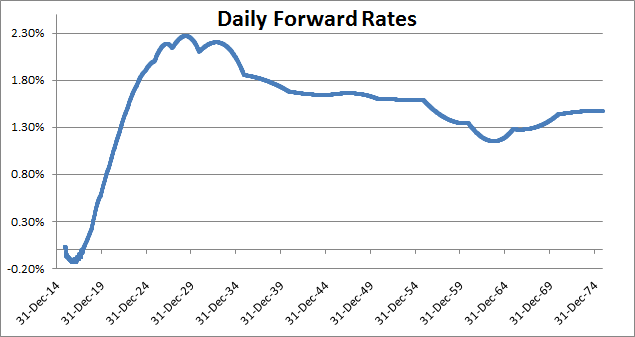
\includegraphics[width=0.7\textwidth]{images/constrainedzero.png}
        \caption{Smooth forward rates obtained through Kruger's constrained cubic interpolation on zero rates.}
        \label{fig:constrainedzero}
        \end{figure}
        
        \begin{figure}[!h]
        \centering
        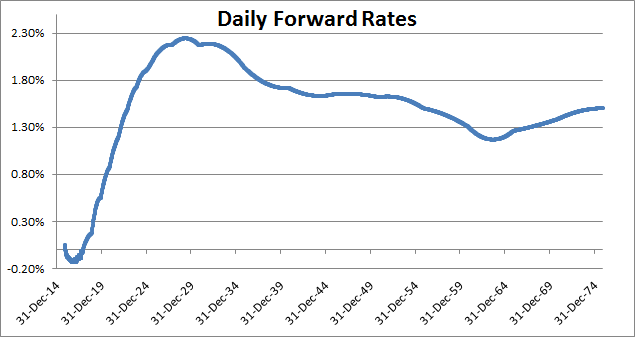
\includegraphics[width=0.7\textwidth]{images/constrainedlog.png}
        \caption{Smooth forward rates obtained through Kruger's constrained cubic interpolation on log-discounts.}
        \label{fig:constrainedlog}
        \end{figure}
        
        \subsection{Monotonic Cubic Natural Spline interpolation: The Hyman Scheme} \label{subsection:3.1.3}
        Cubic spline interpolation methods suffer of well-documented problems, such as spurious inflection points, excessive convexity, lack of locality and wide oscillation that can generate negative forward rates.
        The Hyman's method or {\it Hyman filter} (see \cite{hyman}) attempts to address traditional cubic spline problems in a different way and, as the Figure \ref{fig:stresscase} suggest, can produce smoother forward rates avoiding the issues listed above.
        
        \begin{figure}[!h]
        \centering
        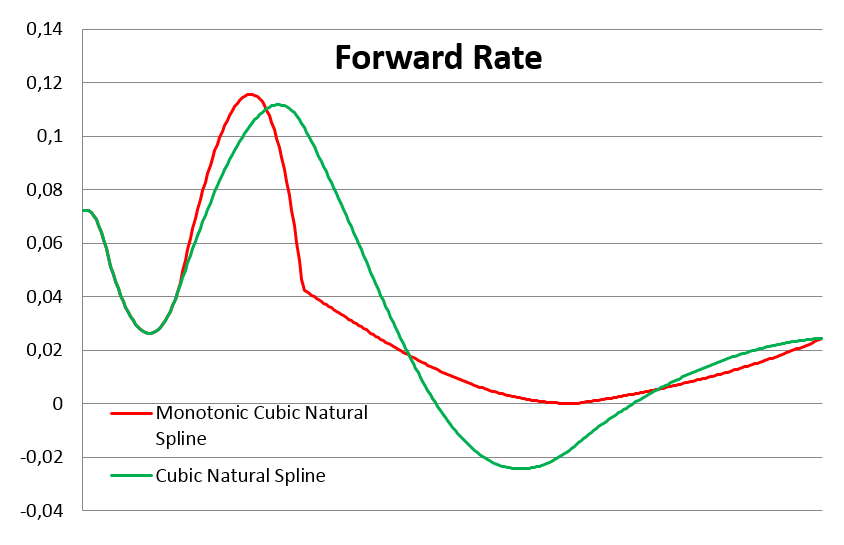
\includegraphics[width=0.7\textwidth]{images/stresscase.png}
        \caption{Hagan and West stress case}
        \label{fig:stresscase}
        \end{figure}
        The Hyman's filter could be applied to any cubic interpolation scheme, for example the cubic natural spline one, to preserve monotonicity. In case of $C^{2}$ interpolation schemes the Hyman filter ensures monotonicity at the expenses of the second derivative of the interpolated function which will no longer be continuous in the points where the filter has been applied.\\
        Let's briefly sketch how Hyman filter works. When input data are locally monotone (three successive increasing or decreasing points), if the chosen interpolating function is already monotonic, the Hyman filter leaves it unchanged preserving all of its original features (and, as a consequence, without introducing any distortion), otherwise it changes the slopes locally just enough to guarantee monotonicity. When the data are not locally monotone, instead, the interpolated function will have a maximum/minimum at the node. Maximum and minimum points are allowed also between pillars. The effect of Hyman Filter applied to Cubic Natural Spline Interpolation on zero rates and on the logarithm of discount factors is shown in Figures \ref{fig:hymanzero} and \ref{fig:hymanlog}. Looking at the smoothness of forward rates, it's clear that this is the best approach from a forward rate smoothness point of view.\\
        
        \begin{figure}[!h]
        \centering
        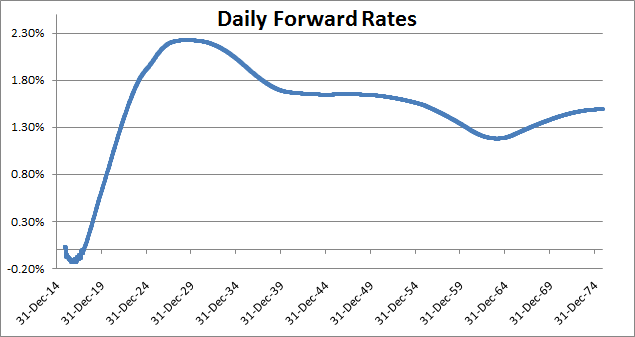
\includegraphics[width=0.7\textwidth]{images/hymanzero.png}
        \caption{Monotonic Cubic Natural Spline interpolation on zero rates.}
        \label{fig:hymanzero}
        \end{figure}
        
        \begin{figure}[!h]
        \centering
        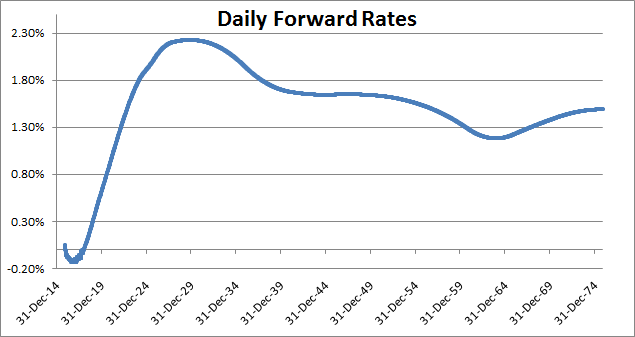
\includegraphics[width=0.7\textwidth]{images/hymanlog.png}
        \caption{Monotonic Cubic Natural Spline interpolation on log-discount Factors.}
        \label{fig:hymanlog}
        \end{figure}
        
        \newpage
        \subsection{Mixed Interpolation} \label{subsection:3.1.4}
        Summing up, it has been previously discussed that the overnight case is the only one where curve's smoothness is not strictly required in the short therm section because market evidence shows that the overnight curve tends to be piecewise constant between ECB monetary policy meeting dates (generally till 1 year and a half from spot date). The best way to replicate this kind of behaviour, as seen in \ref{subsection:3.1.1} is to use a Log-Linear interpolation which produces flat forwards between pillars. After the last ECB dated OIS, however, assuming a piecewise constant curve is no more reasonable; so it becomes necessary to use again an interpolation technique which produces smooth forward rates (like the cubic splines discussed in \ref{subsection:3.1.2} and \ref{subsection:3.1.3}). Since using a Log-Linear or a Cubic interpolation for the whole curve leads, in both cases, to distortions, the best way to model the overnight curve behaviour is by means of {\itshape Mixed Interpolation} which, as the same suggest, permits to mash two kind of interpolation following two different methods:
        
        \begin{itemize}
            \item The {\itshape Split Range} approach which consists in interpolate till a pre-determined pillar (from now called the {\itshape Switch Pillar}) using an interpolation technique and to interpolate using another techniques after that.
            \item {\itshape Share Range} approach it is a bit more sophisticated and consists in interpolate two times the whole curve; the first time using a techniques and the second time using the other one and then merge the obtained curves in the pre-determined switch pillar. 
        \end{itemize}
        Coming back to the previous sections, it has been discussed that the best way to obtain a piecewise constant curve is by means of a Linear interpolation on log-discounts and the best way to obtain smooth forward rates is to use a Monotonic Cubic Natural Spline on log-discounts with the Hyman filter. So, it makes sense to build a Mixed Interpolation which uses a Log-Linear interpolation before the switch pillar and a Natural Spline with Hyman filter after that. \\
        The results of this approach are shown in Figure \ref{fig:mixedinterpsplit} and \ref{fig:mixedinterpshare}. \\
        
        \begin{figure}[!h]
        \centering
        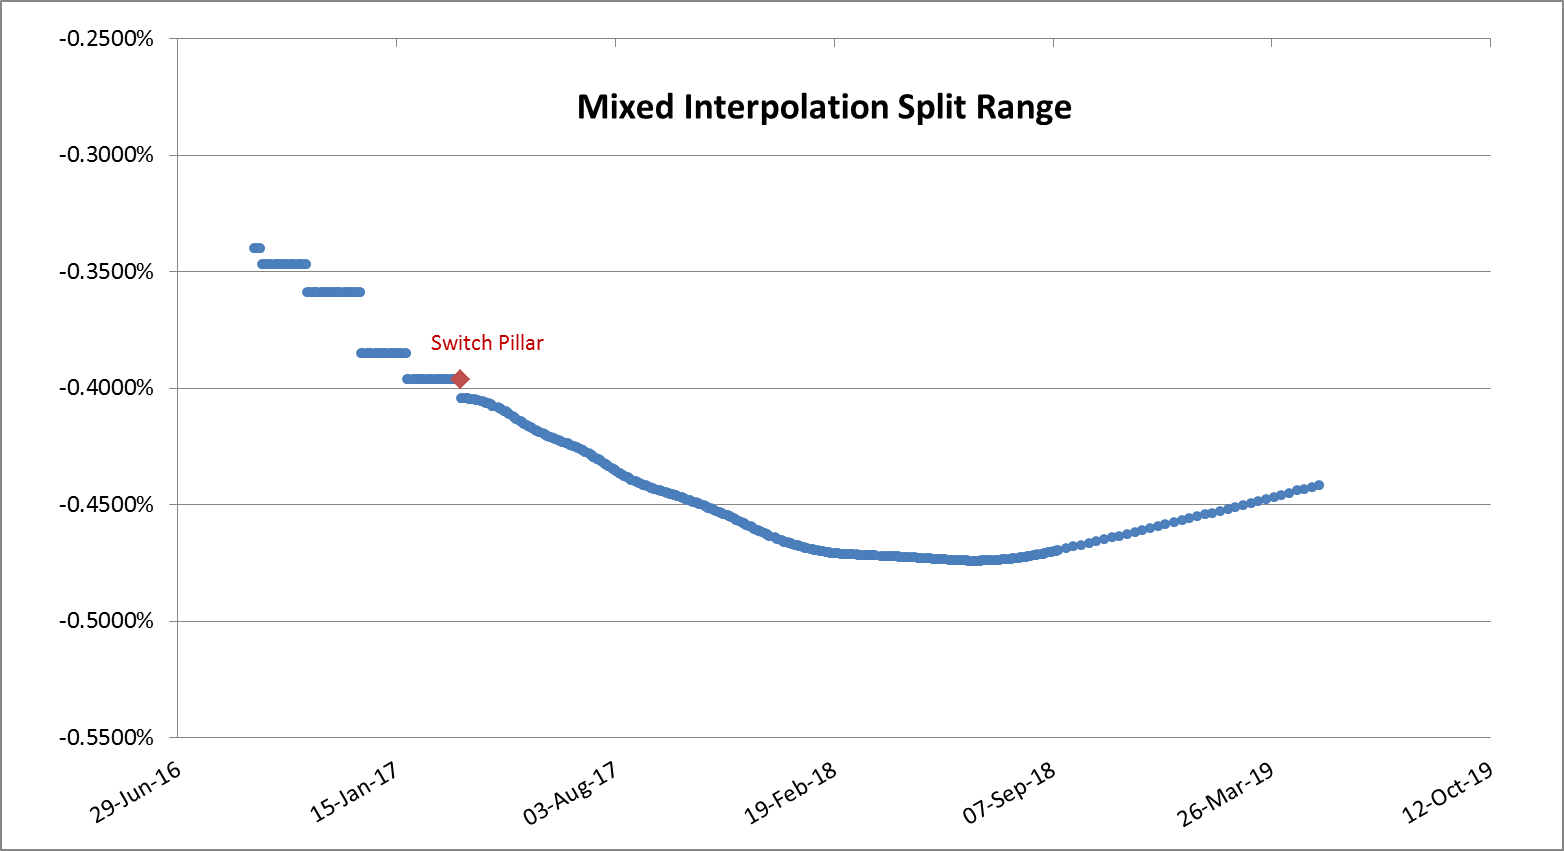
\includegraphics[width=0.7\textwidth]{images/mixedinterpsplit.png}
        \caption{Mixed forward rates obtained through a Mixed interpolation with slit range approach.}
        \label{fig:mixedinterpsplit}
        \end{figure}
        
        Analyzing the image it is straightforward to understand that this process produces a mixed curve behaviour which is flat before the switch pillar and smooth after it.
        
        \begin{figure}[!h]
        \centering
        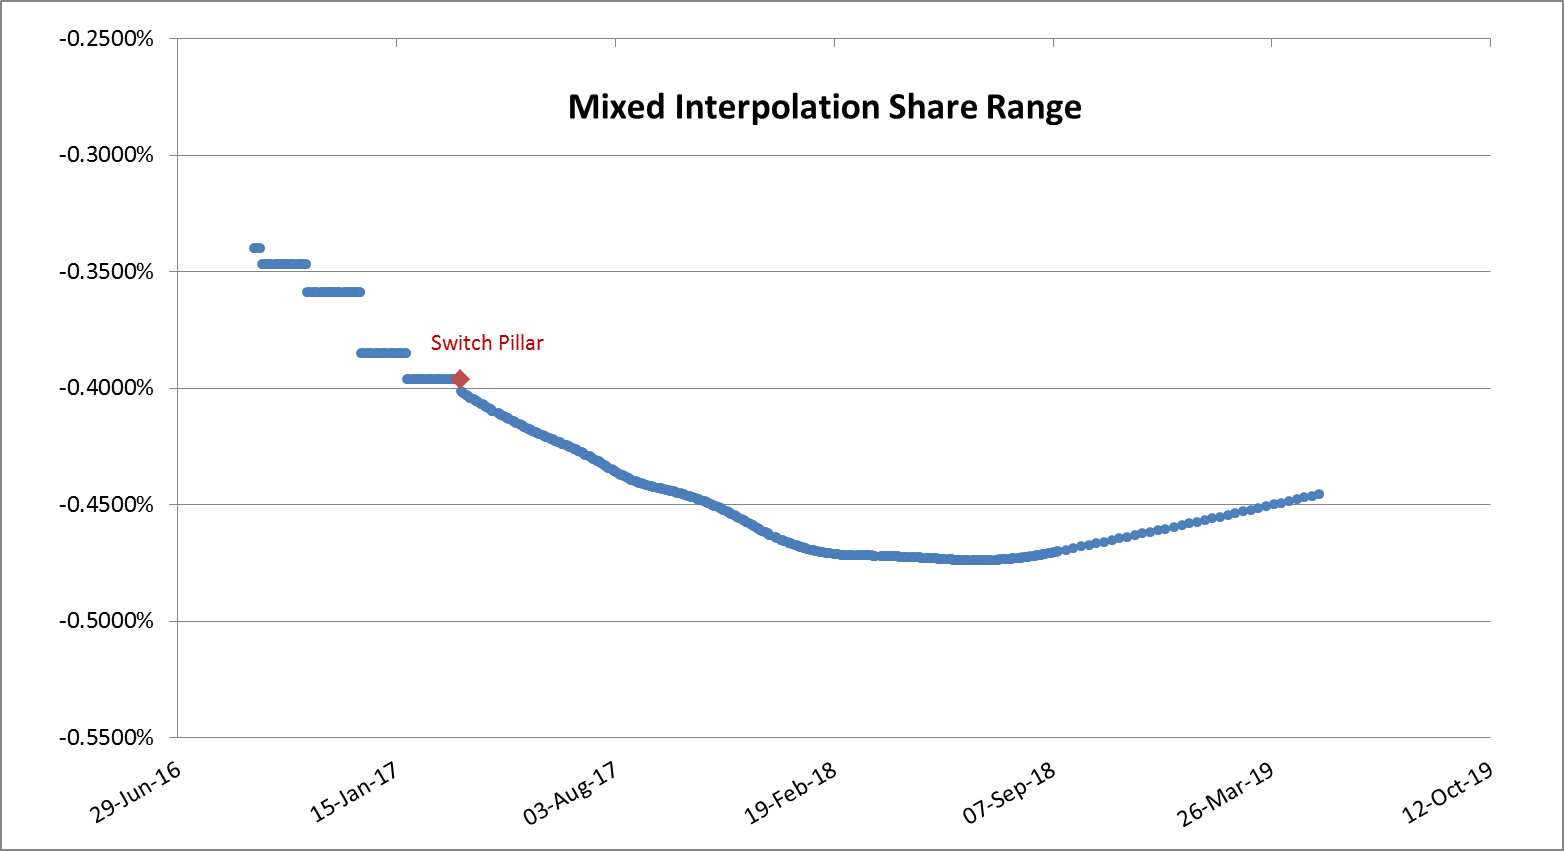
\includegraphics[width=0.7\textwidth]{images/mixedinterpshare.png}
        \caption{Mixed forward rates obtained through a Mixed interpolation with share range approach.}
        \label{fig:mixedinterpshare}
        \end{figure}
        
        \newpage
        As visible in the previous figures the two approaches produce a very similar behaviour. Finally, a repricing error analysis is shown in Figure \ref{fig:repricingmixed}.  \\
        
        \begin{figure}[!h]
        \centering
        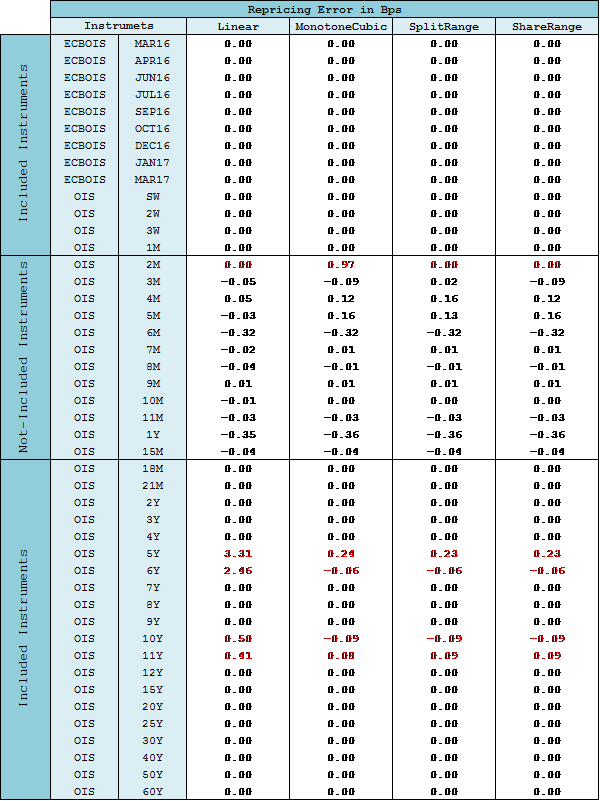
\includegraphics[width=0.6\textwidth]{images/repricingmixed.png}
        \caption{Repricing errors on out-of-curve OIS using a linear interpolation for the whole curve (first column), a share range mixed interpolation (second column) and a split range mixed interpolation (last column).}
        \label{fig:repricingmixed}
        \end{figure} 
        The aim of this analysis is to demonstrate that the mixed interpolation is the best way to interpolate the overnight curve looking to the curve goodness, expressed in out-of-curve OIS repricing errors. In order to do that, a Log-Linear approach for the whole curve, a Mixed Log-linear/Hyman share range approach and a Mixed Log-linear/Hyman split range approach have been compared. Figure \ref{fig:repricingmixed} shows that the three methods produce almost the same results in the short term section curve but in the long term section the repricing errors tend to diverge due to the fact that a piecewise constant interpolation becomes less and less accurate as the instrument maturity increase.  \\
        For this reasons, this work suggest that the mixed interpolation is the best way to interpolate the overnight curve and it has also the advantage to permits the usage of a {\it Forward Stub} in order to fix the overlapping problem that it will be discussed in next section.
         
    \section{Forward Stub for overlapping Instruments} \label{section:3.2}
    This section is devoted to the presentation and solution of a particular overnight curve problem due to the manage of the first ECB dated OIS. This kind of instruments are forward start OIS that must be included in the curve calibration because of their liquidity. The problem occurs since spot starting OIS maturity dates,in most of the cases, does not coincide with the settlement date of the first ECB OIS and this leads to a situation in which there are two solutions but either of them produces good results:
    
     \begin{itemize}
         \item{} A possibility is to include all spot starting OIS taking no care of the fact that certainly one of them will have an overlapping maturity date with the forward start ECB OIS (except for the lucky case in which a spot starting OIS maturity coincides with the ECB dates OIS settlement but this situation can only happens one day for each instrument). This solution's benefit is that the ON curve will be totally covered because the bootstrap algorithm can manage a sequence of maturities which permits a "pillar-to-pillar" standard bootstrap. Otherwise this choice implies that there will be a short time-frame presenting overlapping instruments as visible in Figure \ref{fig:overlapping}.
         
        \begin{figure}[!h]
        \centering
        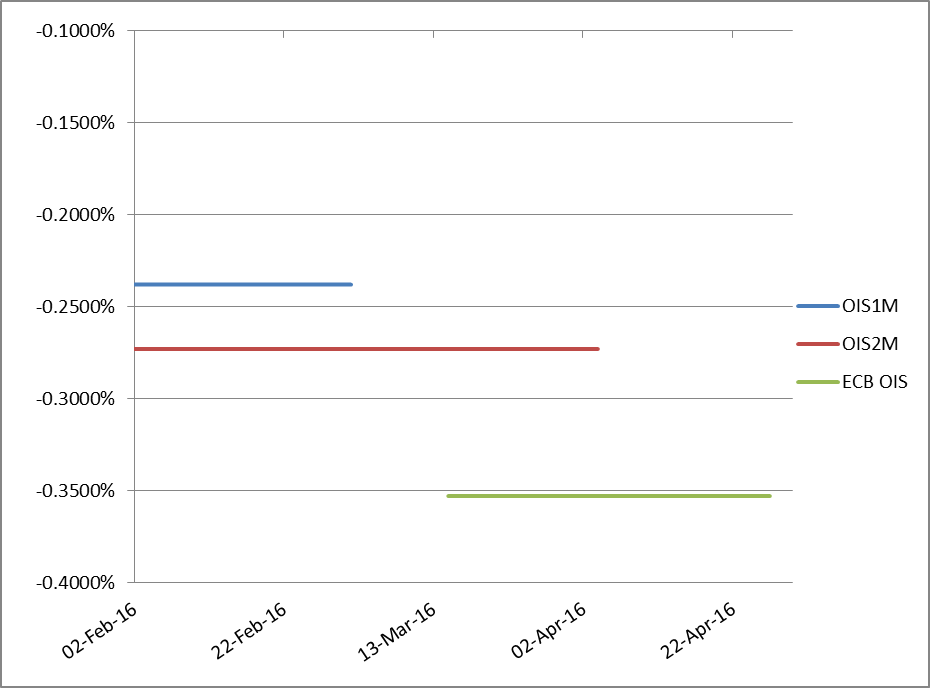
\includegraphics[width=0.7\textwidth]{images/overlapping.png}
        \caption{The overlapping solution using 2 February 2016 values.}
        \label{fig:overlapping}
        \end{figure}

        The example shows that OIS with 2-month maturity ({\it 4 April 2016}) overlaps the first ECB OIS with settlement ({\it 16 March 2016}). This 18 days year fraction cause oscillations in the curve's shape and, as a consequence, an impact on not included instruments repricing errors. This errors are also deeply connected to the first section curve's shape; in fact this solution may leads to negligible repricing errors only if spot starting OIS and first ECB OIS presents close values (which means that the first curve section tends to be flat). Otherwise, empirical evidence shows that, sometimes, market idiosyncrasies can affect first section curve's shape making it highly downward/upward sloping (as the Figure \ref{fig:overlapping} suggest). In this particular cases also the overlapping solution fails leading to relevant errors as it will be shown in \ref{subsection:3.2.2}.
        
        \item{} Another possible solution may be to exclude from the bootstrap the overlapping OIS (the 2-month maturity one in reference to the preceding example). The benefit of this choice is to avoid overlapping instruments but implies that there will be a not covered curve section, as visible in Figure \ref{fig:exclude}, in which the bootstrap algorithm does not have any information related to the curve shape. The impact of this solution on repricing errors is very bad and so it is not advisable to use it. 
        
        \begin{figure}[!h]
        \centering
        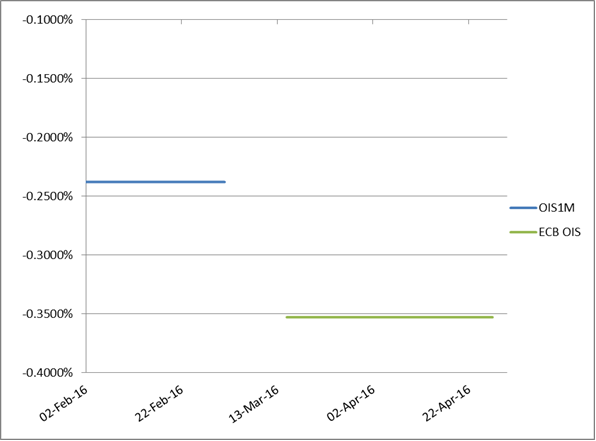
\includegraphics[width=0.6\textwidth]{images/exclude.png}
        \caption{The excluding solution using 2 February 2016 values.}
        \label{fig:exclude}
        \end{figure}
        
        This answers are not satisfactory and seems that there is no solution taking advantage of the only market instruments.\\
        This work's suggestion is to create a forward "Meta-Instrument", from now called {\it Stub}, which value can be derived from available market quotes as it will be discussed in next section.
        
        \end{itemize}

        \subsection{Implied value calculation} \label{subsection:3.2.1}
        Let's suppose now to be in the situation described in Figure \ref{fig:exclude} in which there is a not covered curve's section. The Stub quote represents a forward rate which starts from the last not-overlapping instrument's (in the previous example the OIS1M) maturity date and ends in the first ECB Dated settlement date.\\
        
        \begin{figure}[!h]
        \centering
        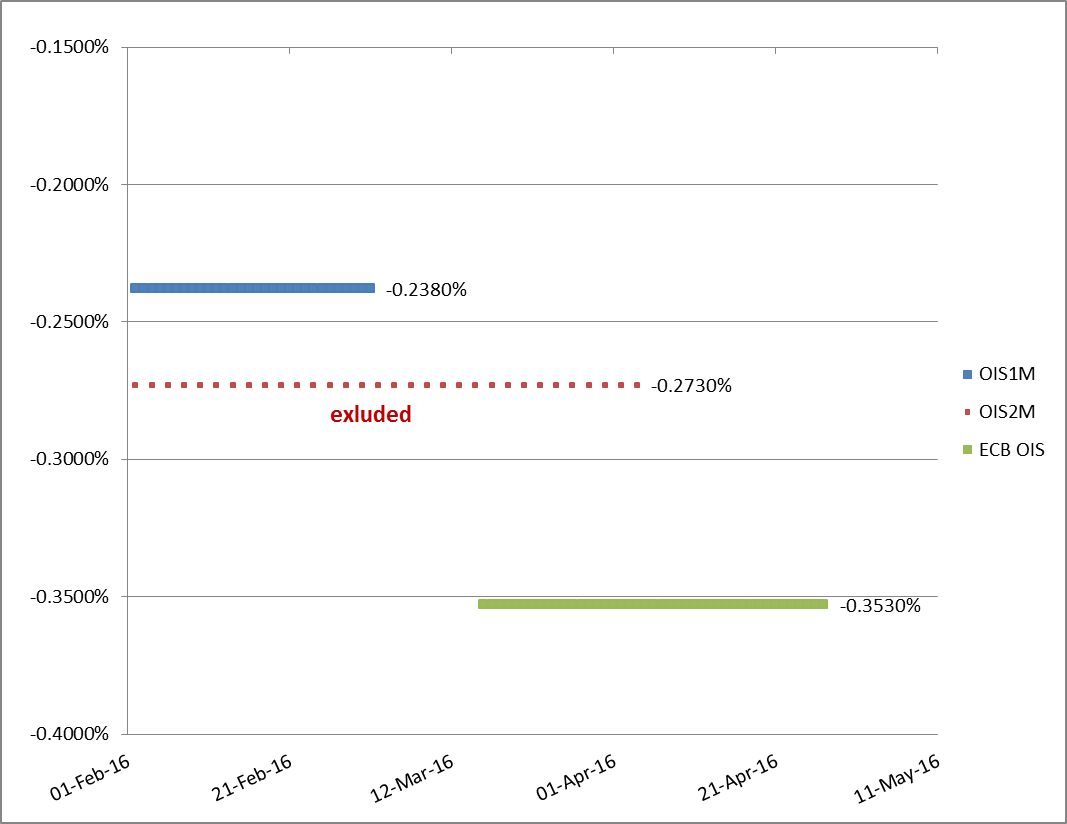
\includegraphics[width=0.6\textwidth]{images/excluded2.png}
        \label{fig:excluded2}
        \end{figure}
        The Stub forward rate is implied in the market and can be derived assuming a no-arbitrage condition. In order to not introduce arbitrages, it is necessary to obtain the Stub quote imposing that the excluded instrument must be repriced exactly (OIS2M in above Figure). In order to replicate the OIS2M value the following relationship must hold:
        
        $$e^{\int_{0}^{t\ped{1}} f_{inst}ds} \cdot e^{\int_{t\ped{1}}^{t\ped{2}} f_{inst}ds} \cdot e^{\int_{t\ped{2}}^{t\ped{3}} f_{inst}ds} = e^{\int_{0}^{t\ped{3}} f_{inst}ds}$$
        where: 
        $$t\ped{1} = \mbox{Last non-overlapping instrument's maturity in year fraction}$$
        $$t\ped{2} = \mbox{First ECB Dated OIS settlement date  in year fraction}$$
        $$t\ped{3} = \mbox{Overlapping instrument's maturity date in year fraction}$$
        $$f_{inst} = \mbox{Instantaneous forward rate}$$
        
        \begin{figure}[!h]
        \centering
        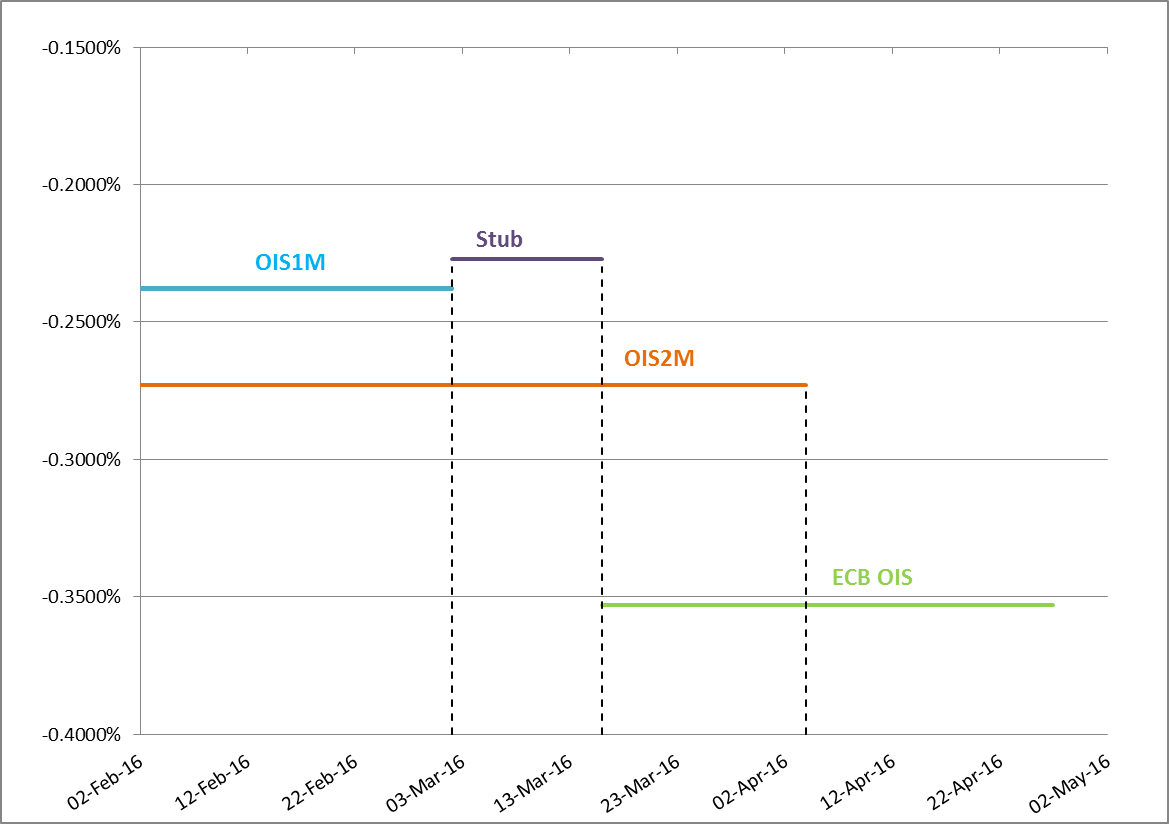
\includegraphics[width=0.6\textwidth]{images/stub.png}
        \caption{The Stub solution using 2 February 2016 values.}
        \label{fig:stub}
        \end{figure}
        As visible in Figure \ref{fig:stub}, no-arbitrage condition implies that investing in OIS1M ({\it blue line}), Stub ({\it violet line}) and in ECB OIS till the OIS2M maturity ({\it green line}) must be equal to investing in OIS2M ({\it orange line}). In this situation, the Stub implied value can be easily calculates as:\\
        
        $$ e^{\int_{t\ped{1}}^{t\ped{2}} f_{inst}ds} = \frac{e^{\int_{0}^{t\ped{3}} f_{inst}ds}}{e^{\int_{0}^{t\ped{1}} f_{inst}ds} \cdot e^{\int_{t\ped{2}}^{t\ped{3}} f_{inst}ds}} $$
        \\
        Assuming simple compounding:\\
        
        $$ \mbox{{\it Stub}} = \frac{[\frac{(1+F\ped{0 x t\ped{3}} \cdot \tau\ped{0 x t\ped{3}})}{(1+F\ped{0 x t\ped{1}} \cdot \tau\ped{0 x t\ped{1}}) \cdot (1+F\ped{t\ped{2} x t\ped{3}} \cdot \tau\ped{t\ped{2} x t\ped{3}})}-1]}{\tau\ped{t\ped{1} x t\ped{2}}}$$\\
        Introducing in the calibration this forward Stub improve consistently the overnight curve goodness avoiding unwanted distortion and oscillation as will be shown in next section. Otherwise, this solution can be implemented only if the bootstrap algorithm uses a log-linear interpolation for the short-term section of the curve. Interpolating log-linearly the overnight curve becomes piecewise constant, as seen in \ref{subsection:1.3.1}, and this assumption permits to derive the $e^{\int_{t\ped{2}}^{t\ped{3}} f_{inst}ds}$ value that must be equal to ECB OIS market quote. The good news is that, as seen in \ref{section:3.1.4}, the best practise to interpolate the ON curve is by means of a mixed interpolation, which interpolates log-linearly the short term section of the curve. It is also important to underlying that the Stub algorithm produces good results also in limit cases as, for example, when $\tau\ped{t\ped{1} x t\ped{2}} \longrightarrow \frac{1}{365}$ that represents the particular case in which the Stub quote duration is just 1 day.\\
        Finally, during a year, there surely happen a particular scenario in which, since the first ECB OIS fixing becomes earlier and earlier, the discarded spot instruments is the first spot starting
        OIS. This case implies that the so called "forward Stub" it is not forward start anymore because it becomes a spot instrument which covers the year fraction: $\tau\ped{0 x t\ped{1}}$ (where $t\ped{1}$ is the first ECB OIS fixing date).
        
        \newpage
        In this case, the "spot stub" implied value is:
        
         $$ \mbox{{\it Stub}} = \frac{[\frac{1+F\ped{0 x t\ped{2}} \cdot \tau\ped{0 x t\ped{2}}}{1+F\ped{t\ped{1} x t\ped{2}} \cdot \tau\ped{t\ped{1} x t\ped{2}})}-1]}{\tau\ped{t\ped{0} x t\ped{1}}}$$
        
        \subsection{Impact on Curve and Repricing Errors} \label{subsection:3.2.2}
        In the previous section it has been presented a particular ON curve problem and 3 possible ways to solve it. Let's start from the worst one, namely the solution in which the overlapping instrument is excluded leaving a non-covered curve's section. With this approach the curve obtained is represented in the underlying figure:\\
        
        \begin{figure}[!h]
        \centering
        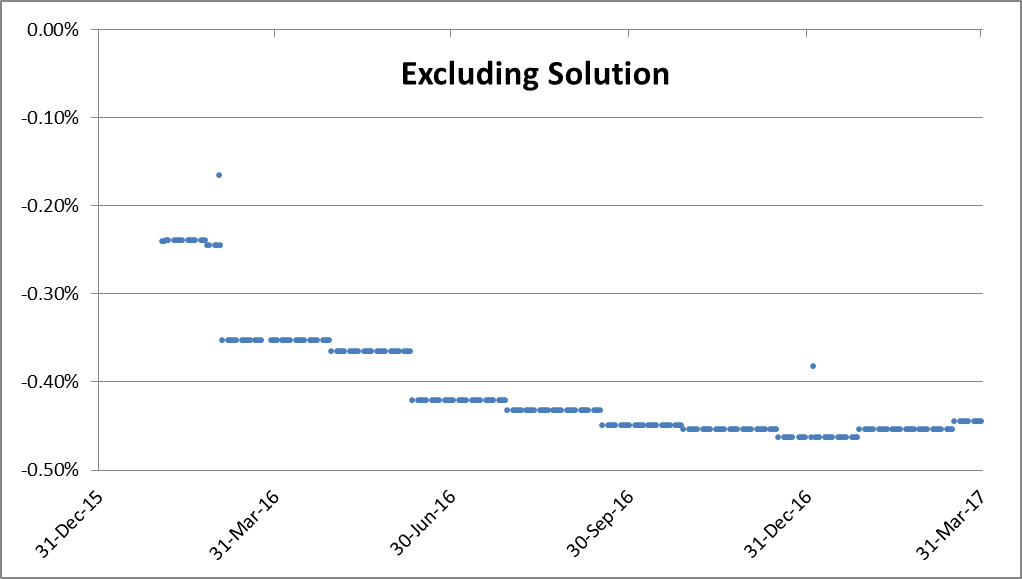
\includegraphics[width=0.7\textwidth]{images/excludingcurve.png}
        \caption{ON Curve excluding overlapping instrument (Evaluation date 2 February 2016).}
        \label{fig:excludingcurve}
        \end{figure}
        
        This solution's big problem is that the bootstrap algorithm extrapolate backward from ECB Dated market quote the non-covered curve's part leading to high distortions especially when preceding instrument and ECB OIS quotes are distant.\\
        A better solution can be including all spot starting OIS even if one of them will certainly be overlapping. This approach is described in next figure:\\
        
        \begin{figure}[!h]
        \centering
        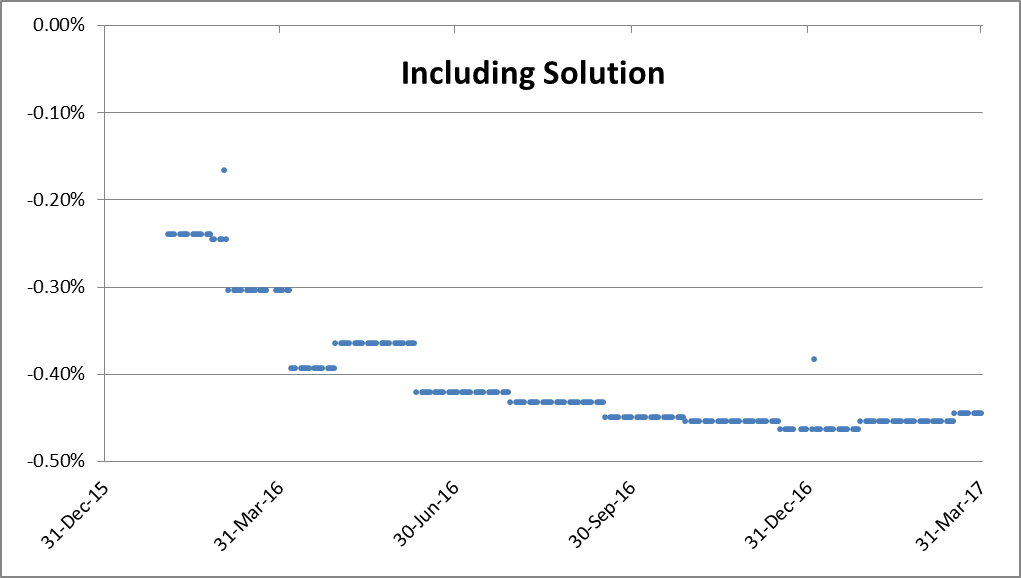
\includegraphics[width=0.7\textwidth]{images/includingcurve.png}
        \caption{ON Curve including overlapping instrument (Evaluation date 2 February 2016).}
        \label{fig:includingcurve}
        \end{figure}
        
        As it will be shown soon, this solution produces distortions due to the fact that the calibration will introduce strange oscillations in order to reprice the overlapping instrument. In fact, the Figure \ref{fig:includingcurve}, shows how the curve is pushed down till $-0.40\%$ and then turns back to the ECB OIS level. It is quite obvious that this strange curve's behaviour is not due to market quotes but to calibration's discrepancy resulting from the overlapping section. Finally, let's present the forward Stub solution in the underlying figure:\\
        
        \begin{figure}[!h]
        \centering
        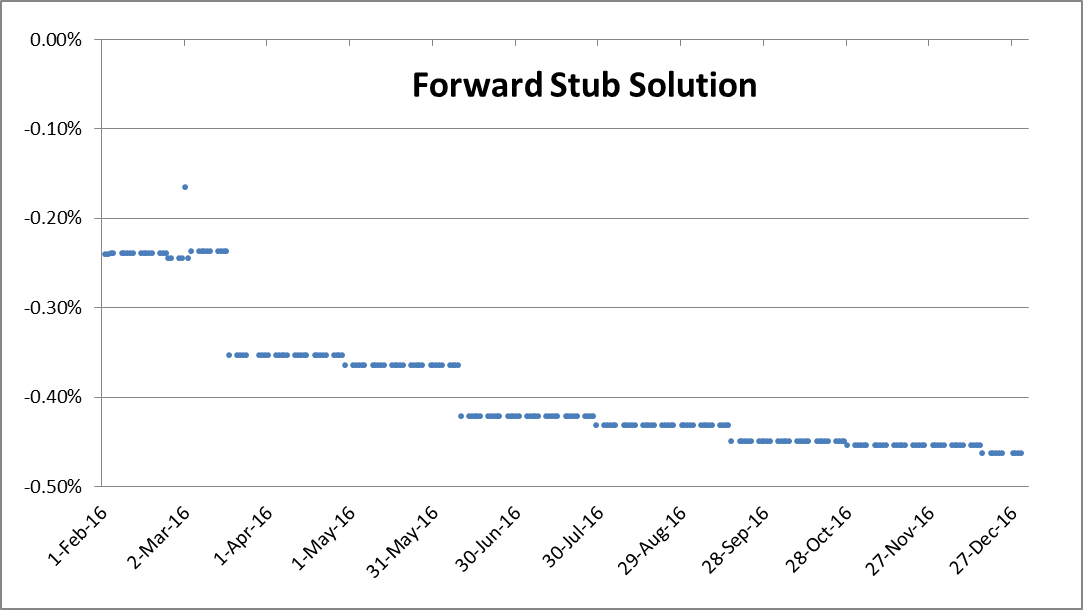
\includegraphics[width=0.7\textwidth]{images/stubcurve.png}
        \caption{ON Curve including forward Stub (Evaluation date 2 February 2016).}
        \label{fig:stubcurve}
        \end{figure}
        
        \newpage
        As visible, there are no wide oscillation in the curve's shape and the repricing errors analysis, represented in Figure \ref{fig:errors}, shows that this approach is the one which minimize all out-of-curve instruments, ensuring also the perfect reprice of the overlapping instrument excluded.
        
        \begin{figure}[!h]
        \centering
        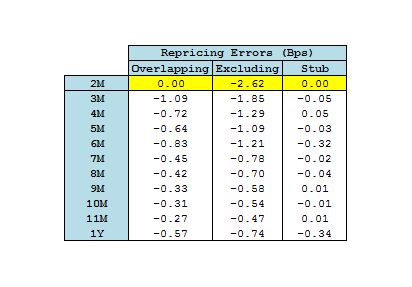
\includegraphics[width=0.6\textwidth]{images/errors.png}
        \caption{Repricing errors summary for all possible solutions.}
        \label{fig:errors}
        \end{figure}
        
        \begin{figure}[!h]
        \centering
        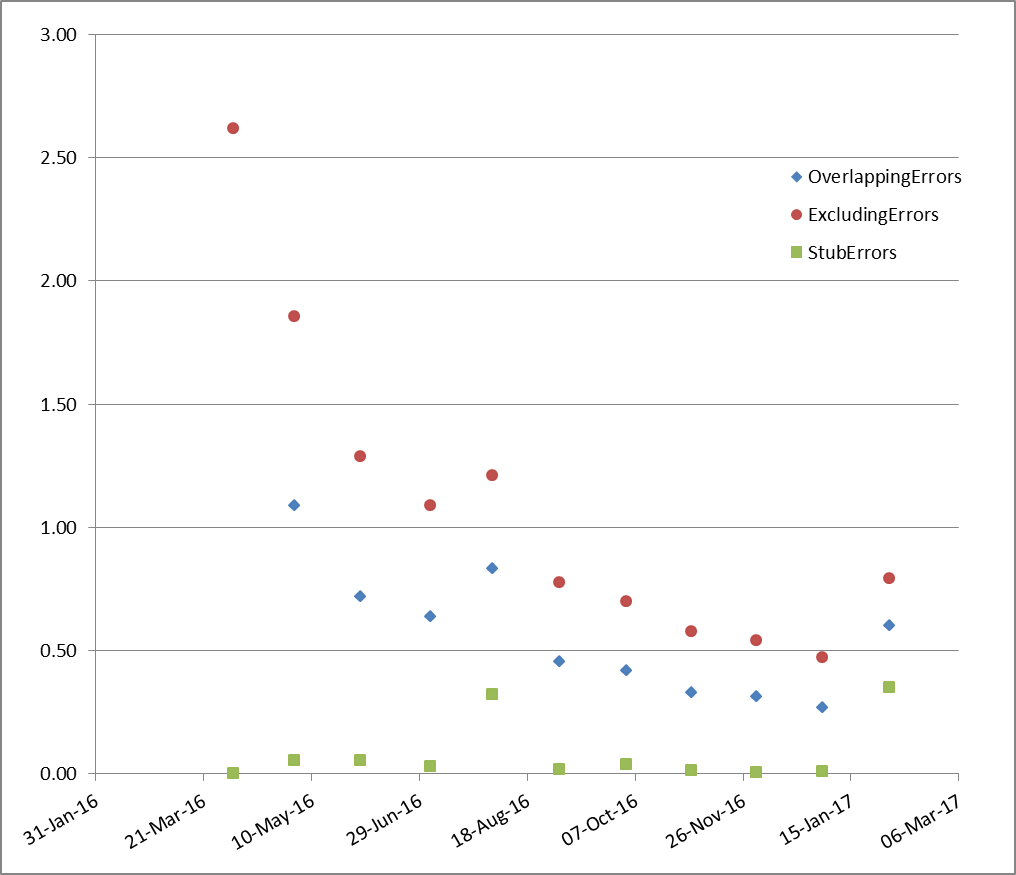
\includegraphics[width=0.7\textwidth]{images/repricingimage.png}
        \caption{The minimization of all out-of-curve instruments repricing errors (in bps) using the Stub solution.}
        \label{fig:repricingimage}
        \end{figure}
        
    \section{Jumps Inclusion} \label{section:3.3}
        \subsection{The EUR market case: Positive Jumps} \label{subsection:3.3.1}
        \subsection{The GBP and USD market case: Negative Jumps} \label{subsection:3.3.2}
        
    \section{Fed Funds Arithmetic Average Coupon OIS} \label{section:3.4}
    From the previous section the subject have been moved to foreign currency overnight curve calibration. This part aims to discuss how the US dollar overnight yield curve (USDON) can be improved including in the bootstrap the Fed Funds (FF) arithmetic OIS instead of the simple OIS indexed to the Fed Funds rate. This is a recommendable practice due to the fact that arithmetic OIS are traded in the dealer's market more actively and so, fore the liquidity criteria discussed in \ref{section:2.1}, it is better to include them in the calibration algorithm.
    
        \subsection{Fed Funds OIS Vs. Arithmetic-LIBOR basis swap} \label{subsection:3.4.1}
        FF-OIS, as already discussed in \ref{subsection:2.1.2}, are particular IRS which floating-leg pays the daily compounded FF rate. In a interest rate basis swap (IRBS), instead, two different floating rates in the same currency are exchanged which can be, for example, two LIBORs with different tenors. Arithmetic-LIBOR, so, are basis swaps which exchange the FF rate on a leg and a LIBOR rate on the other. In derivative products like swaps the FF rates, as the EUR overnight ones, are never paid on a daily basis but paid collectively in a single coupon. The difference between FF-OIS and Arithmetic-LIBOR basis swaps is that, while in FF-OIS coupons are done on a daily compounded basis, in Arithmetic-LIBOR basis swaps are built doing an arithmetic average. This calculation difference leads to some complications which implies two convexity adjustment which derivation will be discuss Section \ref{subsection:3.4.5}.\\
        Expressing the previous concept in formulas, it is possible to define the daily compounded FF-OIS rate for the period $(t\ped{1},t\ped{2})$ as:
        
        $$R^{OIS}(t\ped{1},t\ped{2}) = \frac{1}{\tau(t\ped{1},t\ped{2})} \left[\prod_{k=1}^{K} (1+\tau\ped{k}r\ped{k})-1\right]$$\\
        While the arithmetic average Fed Funds rate is sampled as:\\
        $$R^{Arithm}(t\ped{1},t\ped{2}) = \frac{\sum_{k=1}^{K} \tau\ped{k}r\ped{k}}{\tau(t\ped{1},t\ped{2})}$$\\
        Where $r\ped{k}$ is the effective ON rates fixed for the period $(t\ped{1},t\ped{2})$ and $\tau\ped{k}$ is the corresponding year fraction calculated in {\it Actual/360}. Since $\tau(t\ped{1},t\ped{2})$ is the year fraction related to the whole interest period, it is straightforward to understand that $\tau(t\ped{1},t\ped{2}) = \sum_{k=1}^{K}\tau\ped{k}$.\\
        So, assuming a notional equal to $N$, the interest paid by the FF-OIS for the period $(t\ped{1},t\ped{2})$ is:
        
        $$N * R^{OIS}(t\ped{1},t\ped{2}) * \tau(t\ped{1},t\ped{2}) = N * \left[\prod_{k=1}^{K} (1+\tau\ped{k}r\ped{k})-1\right]$$
        and for the Arithmetic-LIBOR basis swap is:
        $$N * R^{Arithm}(t\ped{1},t\ped{2}) * \tau(t\ped{1},t\ped{2}) = N * \sum_{k=1}^{K}\tau\ped{k}r\ped{k}$$
        
        \subsection{Fed Funds OIS and Arithmetic-LIBOR basis swap valuation} \label{subsection:3.4.2}
        Denoting as $D(t,T)$ the value at maturity $T$ of a collateralized Bond, its payoff can be defined as the conditional expectation at time $T$, under a proper risk-neutral measure $M$, of the average risk-free rate which, for all collateralized interest rate derivatives, can be substituted with the overnight rate (see \cite{hull} for more details). In formula:
        
        $$D(t,T) = E^{M}\ped{t} \left[e^{-\int_t^T r(u)du}\right]$$
        This permits to express the value $V(t,T)$ of a collateralized FF-OIS over the accrual period $(t\ped{1},t\ped{2})$ as:
        
        \begin{equation*}
        \begin{split}
        V^{OIS}(t\ped{1},t\ped{2}) &= E^M \left[e^{-\int_0^{t\ped{2}} r(u)du} \tau(t\ped{1},t\ped{2})R^{OIS}(t\ped{1},t\ped{2})\right] \\
        &= E^M \left[e^{-\int_0^{t\ped{2}} r(u)du} \left[\prod_{k=1}^{K} (1+\tau\ped{k}r\ped{k})-1\right]\right] \\
        &= D(0,t\ped{1})-D(0,t\ped{2})\\
        \end{split}
        \end{equation*}
        so the $t$ forward OIS rate is given by:
        
        $$R_f^{OIS}(t;t\ped{1},t\ped{2}) = \frac{1}{\tau(t\ped{1},t\ped{2})}\left[\frac{D(t,t\ped{1})}{D(t,t\ped{2})}-1\right]$$
        The Arithmetic-LIBOR basis swap present value over the accrual period $(t\ped{1},t\ped{2})$, instead, is given by:
    
        \begin{equation*}
        \begin{split}
        V^{Arithm}(t\ped{1},t\ped{2}) &= E^M \left[e^{-\int_0^{t\ped{2}} r(u)du} \tau(t\ped{1},t\ped{2})R^{Arithm}(t\ped{1},t\ped{2})\right] \\
        &= E^M \left[e^{-\int_0^{t\ped{2}} r(u)du} \left[\prod_{k=1}^{K} \tau\ped{k}r\ped{k}\right]\right] \\
        &\approx E^M \left[e^{-\int_0^{t\ped{2}} r(u)du} \int_{t\ped{1}}^{t\ped{2}} r(u)du\right] \\
        &= D(0,t\ped{2})E^{t\ped2}\left[\int_{t\ped{1}}^{t\ped{2}} r(u)du\right]
        \end{split}
        \end{equation*}
        Where the collateralized Bond value $D(0,t\ped{2})$ with maturity $t\ped{2}$ is the numeraire which permits to move in a forward risk neutral world and $e^{-\int_0^{t\ped{2}} r(u)du}$ is the stochastic discount factor.
    
        \subsection{The geometric average approximation} \label{subsection:3.4.3}
        Katsumi Takada (see \cite{takada}) has shown that, to evaluate Arithmetic-LIBOR basis swap, a geometric approximation can be used. This approach takes advantage of the relationship between simple compounded and continuously compounded rates:
        
        $$1 + R * \tau(t,T) = e^{\tau(t,T)*r}$$
        If $R$ it is assumed to be the overnight rate than the compounded amount between the accrual period $(t\ped{1},t\ped{2})$ is calculated as:
        
        $$\prod_{k=1}^{K}(1+\tau\ped{k}R\ped{k}) = e^{\sum_{k=1}^{K}\tau\ped{k}r\ped{k}}$$
        Where $R\ped{k}$ is the simple compounded ON rate and $r\ped{k}$ is the continuously compounded ON rate which satisfies the relationship expressed before. the previous equation also implies a limiting relationship so that:
        
        $$\lim_{\tau \rightarrow 0}(1+\tau R)^{\frac{1}{\tau}} = e^R$$
        This means that if $\tau$ is enough small like, for example, one day ($\frac{1}{360}$ using a Act/360 convention) then the simple ON rate $R$ approximates reasonably the continuously compounded ON rate $r$. Since the ON rate has a small $\tau$, it is possible to re-write the previous equation:
        $$\prod_{k=1}^{K}(1+\tau\ped{k}R\ped{k}) = e^{\sum_{k=1}^{K}\tau\ped{k}r\ped{k}}$$
        like:
        $$\prod_{k=1}^{K}(1+\tau\ped{k}R\ped{k}) = e^{\sum_{k=1}^{K}\tau\ped{k}R\ped{k}}$$
        So, the Arithmetic-LIBOR basis swap rate can be also re-written as:
        \begin{equation*}
        \begin{split}
        V^{Arithm}(t\ped{1},t\ped{2}) &= \frac{1}{\tau(t\ped{1},t\ped{2})}log\prod_{k=1}^{K}(1+\tau\ped{k}R\ped{k})\\
        &= \frac{1}{\tau(t\ped{1},t\ped{2})}log(1+\tau(t\ped{1},t\ped{2})R^{OIS}(t\ped{1},t\ped{2})) \\
        \end{split}
        \end{equation*}
        This leads to another possible description of the Arithmetic-LIBOR basis swap valuation formula:
        
        \begin{equation*}
        \begin{split}
        V^{Arithm}(t\ped{1},t\ped{2}) &= E^M \left[e^{-\int_0^{t\ped{2}} r(u)du} \tau(t\ped{1},t\ped{2})R^{Arithm}(t\ped{1},t\ped{2})\right] \\
        &= E^M \left[e^{-\int_0^{t\ped{2}} r(u)du} \left[\sum_{k=1}^{K} \tau\ped{k}r\ped{k}\right]\right] \\
        &\approx E^M \left[e^{-\int_0^{t\ped{2}} r(u)du} \left[log\prod_{k=1}^{K} (1+\tau\ped{k}R\ped{k}\right]\right] \\
        &\approx E^M \left[e^{-\int_0^{t\ped{2}} r(u)du} \int_{t\ped{1}}^{t\ped{2}} r(u)du\right] \\
        &= D(0,t\ped{2})E^{t\ped2}\left[\int_{t\ped{1}}^{t\ped{2}} r(u)du\right]
        \end{split}
        \end{equation*}
        In this case, the Airthmetic-LIBOR $t$ forward rate can be defined as:
        $$R_f^{Arithm}(t;t\ped{1},t\ped{2}) = \frac{1}{\tau(t\ped{1},t\ped{2})}E^{t\ped{2}}\left[\int_{t\ped{1}}^{t\ped{2}} ru(du)\right]$$
        Supposing that rates have no volatility, the ON rate $r(u)$ at time $u$ can be replaced by the initial instantaneous forward rate with maturity $u$, $r(0;u)$. In this particular case one of the two convexity adjustment must not be considered anymore and it is possible to derive:
        
        \begin{equation*}
        \begin{split}
        \int_{t\ped{1}}^{t\ped{2}}r(0;u)du &= log\frac{D(0,t\ped{1})}{D(0,t\ped{2})}\\
        &= log(1+ \tau(t\ped{1},t\ped{2})*R_f^{Arithm}(0;t\ped{1},t\ped{2}))
        \end{split}
        \end{equation*}
        Otherwise, plotting $log(1+\tau(t\ped{1},t\ped{2})*R_f^{OIS}(0;t\ped{1},t\ped{2}))$ against $\tau(t\ped{1},t\ped{2})*R_f^{OIS}(0,t\ped{1},t\ped{2})$ it is clear that there is a convexity in Arithmetic-LIBOR coupon relative to FF-OIS coupon as shown in Figure \ref{fig:convexity2}. It is also clear that in any case it results that:
        
        $$\tau(t\ped{1},t\ped{2})*R_f^{OIS}(0,t\ped{1},t\ped{2}) \geq log(1+\tau(t\ped{1},t\ped{2})*R_f^{OIS}(0;t\ped{1},t\ped{2}))$$\\
        except when $R_f=0$ in which the payoffs are equal. For this reason, to avoid any kind of arbitrage, the following relationship must hold:
        
        $$R_f^{Arithm}(0,t\ped{1},t\ped{2}) < \frac{1}{\tau(t\ped{1},t\ped{2})}log(1+\tau(t\ped{1},t\ped{2})*R_f^{OIS}(0;t\ped{1},t\ped{2})) < R_f^{OIS}(0;t\ped{1},t\ped{2})$$
        
        \begin{figure}[!h]
        \centering
        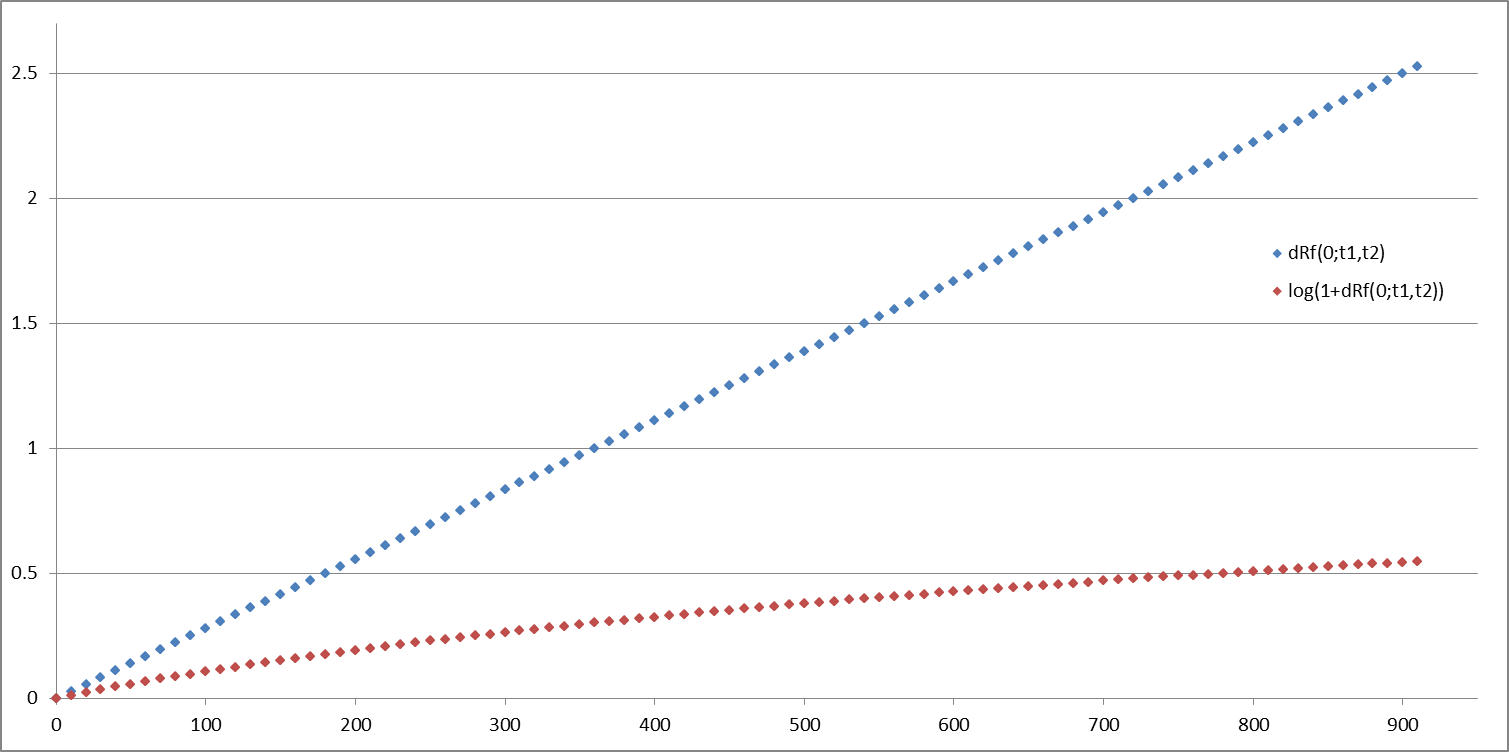
\includegraphics[width=0.7\textwidth]{images/convexity2.png}
        \caption{Also without volatility it emerges another kind of convexity in the two payoffs.}
        \label{fig:convexity2}
        \end{figure}
        In conclusion, it is possible to say that the $R_f^{Arithm}(t;t\ped{1},t\ped{2})$ is smaller than the $R_f^{OIS}(t;t\ped{1},t\ped{2})$ by 2 different convexity adjustment the first of which is static and exists even if there is no volatility. Its value corresponds to:
        
        $$ConvAdj_1 = R_f^{OIS}(0;t\ped{1},t\ped{2}) - \frac{1}{\tau(t\ped{1},t\ped{2})}log(1+\tau(t\ped{1},t\ped{2})*R_f^{OIS}(0;t\ped{1},t\ped{2}))$$
        This is the convexity correction shown in the previous figure. The other convexity adjustment is, instead, dynamic since it is caused by the forward OIS rate volatility and its value is:
        $$ConvAdj_2 = \frac{1}{\tau(t\ped{1},t\ped{2})}log(1+\tau(t\ped{1},t\ped{2})*R_f^{OIS}(0;t\ped{1},t\ped{2})) - R_f^{OIS}(0;t\ped{1},t\ped{2})$$
        The valuation of this second correction term could be performed taking advantage of an Hull \& White short rate model (for more information see \cite{hullwhite}) but its derivation is outside the purposes of this work.
    
        \subsection{Bootstrap methodology and impact on USDON curve} \label{subsection:3.4.4}
        Actually this kind of instruments are quoted as spread $S_T$ against USD Libor 3M, so it is possible to set the following equation:

        \begin{equation*}
        \begin{split}
        \sum_{i=1}^{N} \tau(t\ped{i-1},t\ped{i}) L_f^{3M}(0,t\ped{i-1},t\ped{i})D(0,t\ped{i}) =
        \sum_{i=1}^{N} (V^{Arithm}(t\ped{i-1},t\ped{i}) + \tau(t\ped{i-1},t\ped{i})S_TD(0,t\ped{i}))
        \end{split}
        \end{equation*}
        In order to use these instruments for building the USD overnight rate curve it is necessary to bootstrap this curve together with the 3M Libor forwarding curve but this implies that both curves must be bootstrapped jointly. Because this combined bootstrap could be a bit complex, suppose that swaps USD Libor 3M against fixed rate are quoted in the market. Each market quote represents the fixed rate making the two legs of the swap equal. So, it is possible to substitute the USD Libor 3M with the fixed rate of the specific swap maturing in $T$ and set the following equation: 

        \begin{equation*}
        \begin{split}
        \sum_{i=1}^{N} \tau(t\ped{i-1},t\ped{i})R_T^{3M}D(0,t\ped{i}) = 
        \sum_{i=1}^{N} V^{Arithm}(t\ped{i-1},t\ped{i}) + \tau(t\ped{i-1},t\ped{i})S_TD(0,t\ped{i}))
        \end{split}
        \end{equation*}
        By means of the synthetic instrument above, the USD overnight curve bootstrap can be performed now deriving the equilibrium spread $S_T$ and without the USD Libor 3M forwarding term structure. Therefore, this simplification allows a standard basis swaps bootstrap.\\
        Including the Arithmetic Fed Funds OIS in the calibration has a good impact on USDON curve smoothness as visible in the next two figures.
        
        \begin{figure}[!h]
        \centering
        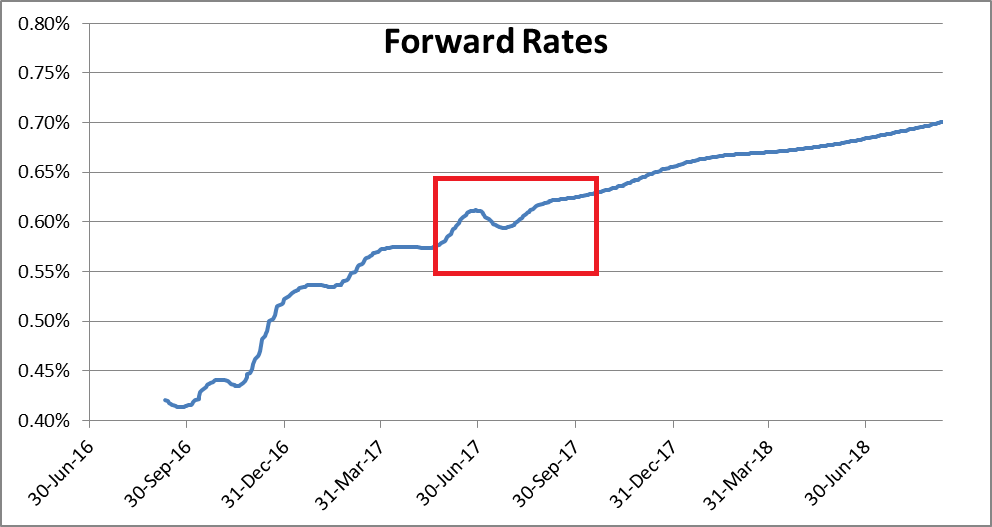
\includegraphics[width=0.7\textwidth]{images/metaoiscurve.png}
        \caption{The USD overnight curve shape without Arithmetic OIS.}
        \label{fig:metaoiscurve}
        \end{figure}
        
        \begin{figure}[!h]
        \centering
        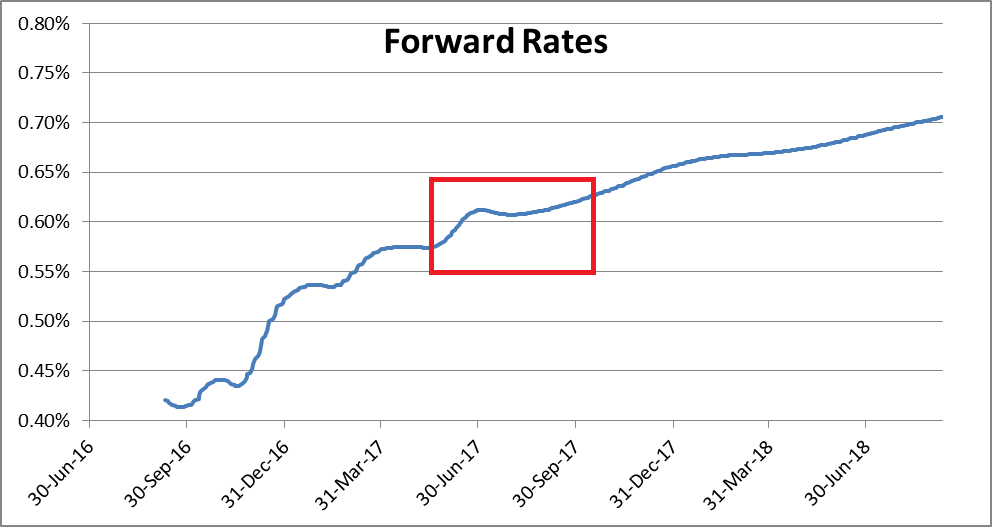
\includegraphics[width=0.7\textwidth]{images/aithmeticcurve.png}
        \caption{The impact of including Arithmetic Fed Funds OIS in the curve calibration.}
        \label{fig:arithmeticcurve}
        \end{figure}
        
        \newpage
        The Arithmetic basis does not exists for tenor less than one year; in fact the impact o the curve's shape is visible from one year after the settlement date and involves a smoother shape.
        
        
%%%CONCLUSION%%%

\chapter*{Conclusion} \label{chap:Concl}
\markboth{\MakeUppercase{Conclusion}}{}
\addcontentsline{toc}{chapter}{Conclusion}

%%%APPENDICES%%%

\newpage
\appendix

\begin{appendices}
  \renewcommand\thetable{\thesection\arabic{table}}
  \renewcommand\thefigure{\thesection\arabic{figure}}
\chapter{Interest Rate Conventions} \label{app:Conv}
With the next two appendices i want to go a step back. The main goal of this work is outline the most important issues related to curve calibration techniques, with particular attention to the overnight one, and this involve a deep understanding of interest rate calculation and conventions but also of the whole set of financial instruments involved in the bootstrap procedure. 
This devoted to introduce some basic and fundamental interest rate rule in order to fix the idea that there are different ways to obtain an interest rate that are strictly connected to the compounding rule chosen, to the way in which time is calculated and to the type of interest.
    \section{Capitalization and Discount Factors} \label{app:capitalization}
    We are all familiar with the concept that cash availability it's a privilege we don't want to give up for free. Of course, everyone who has an amount of money want to be compensated if he decides to lend it and this is the reason why negative interests rates were unthinkable. however, today's index fixings are deeply below zero due to very expansive Central Bank's monetary policy and, in this scenario, a future amount of money worth less than the same amount of money owned today. Aside from negative rates issue, what we need is answer to the questions:
    \begin{description}
        \item{-} What is the future value of a today's amount of money?
        \item{-} What is the present value of a future cash flow?
    \end{description}
    To answer we have to introduce Capitalization and Discount Factors.
    The capitalization factor: $h(R,(t_2-t_1))$ measures the future value, after the year fraction $(t_2-t_1)$ (from now $\tau$) of a unit of currency owned today; instead, the discount factor: $\frac{1}{h(R,\tau)}$ measures the present value of a unit of currency paid after the year fraction $\tau$. This premise is necessary to introduce an important notion that has been true for a long time but not anymore, namely that capitalization factors are an increasing function of time and, consequently, their inverse, the discount factors, are a decreasing function of time.\\
    Naming:\\
    $$D(t) \mbox{ the discount factor in }  t, \mbox{ and:}$$ 
    $$C(t) = \frac{1}{D(t)} \mbox{ the capitalization faction in } t$$\\
    we have that, {\bfseries assuming positive interest rates}:\\
    $$D(t) < 1 \mbox{ for any } t > 0$$
    $$D(t_1) > D(t_2) \mbox{ if } t_1<t_2\mbox{ and:}$$
    $$C(t) > 1 \mbox{ for any } t > 0$$
    $$C(t_1) < C(t_2) \mbox{ if } t_1<t_2\mbox{ and:}$$\\
    As we will see, define the function $h(R,\tau)$ isn't so easy as it seems because the capitalization formula can be measured in different ways.
    Changing parameters has a strong impact on capitalization/discount factors; therefore, it's fundamental to take confidence with all kinds of parametrization starting from compounding rules.
    \section{Compounding Rules} \label{app:compoundingrules}
    For compounding rule we mean a method to calculate the future value of an amount of money. The easier way to describe $h(R,(t_2-t_1))$ function is to use the {\itshape simple compounding scheme}.
        \subsection{Simple Compounding} \label{app:simple}
        This scheme implies that: $$ I = N*R*\tau$$ $$N+I=N*(1+R*\tau)$$ where $I$ is the interest amount in $t_2$ and $N$ is the notional at the beginning of the accrual period ($t_1$). Accordingly, the Capitalization Factor in simple compounding is: 
        $$C(t) = h(R,\tau) = (1+R*\tau)$$\\
        and the Discount Factor is: 
        $$D(t) = \frac{1}{h(R,\tau)} = \frac{1}{(1+R*\tau)}$$
        Therefore, the capital grows linearly during time because interest amounts are not capitalized to produce other interests.
        \subsection{Compounded Interest Rate} \label{app:compounded}
        In this scheme interests are compounded $m$ times per year for $\tau$ years at rate R. So, investing a notional N produce at the end of the accrual period:
        $$N*\left(1+\frac{R}{m}\right)^{m\tau}$$   
        The compounded Capitalization and Discount Factors, therefore, are:
        $$C(t) = h(R,\tau) = \left(1+\frac{R}{m}\right)^{m\tau}$$ 
        $$D(t) = \frac{1}{h(R,\tau)} = \left(1+\frac{R}{m}\right)^{-m\tau}$$
        Using the compounded scheme means that, every $m$ times the interest is compounded, the capital accrued become the new initial capital and this means that interests are producing other interests. 
        \subsection{Continuous Compounding} \label{app:continuous}
        This compounding rule can be view as a particular case of the preceding one in which we imagine to compound more and more frequently simply taking the limit of $m$ tending to infinity. Expressing this concept in formulas the continuously compounded interest rate is given by:
        $$\lim_{m\rightarrow+\infty} N*\left(1+\frac{R}{m}\right)^{m\tau} = N*e^{R\tau}$$
        Hence, the Capitalization and Discount factors in continuous compounding are:
        $$C(t) = h(R,\tau) = e^{R\tau}$$ 
        $$D(t) = e^{-R\tau}$$
        A good approximation of the continuous interest is to do the daily compounded interest rate. Assuming a year composed by 365 days we have that:
        $$e^{R\tau} \approx \left(1+\frac{R}{365}\right)^{-365\tau}$$
    \section{Day-Count Conventions} \label{app:daycounter}
    After having specified how the interest can be compounded, we have to describe how we can measure the year fraction $\tau = (t_2-t_1)$. For a easier computation, market participants use different kind of conventions called {\itshape Day Counter}; let's describe the most popular:
    \begin{itemize}
    \item \textit{Actual/360} : where \textit{Actual} is the number of days between the two dates.
    $$Actual/360 = \frac{d_2-d_1}{360}$$
    \item \textit{Actual/365 (fixed)}: where \textit{Actual} is defined as before and 365 is used even in a leap year.
    $$Actual/365 (fixed) = \frac{d_2-d_1}{365}$$
    \item \textit{30/360}: where the numerator is obtained as:
    $$360 \cdot(Y_2-Y_1)+30*(M_2-M_1)+(d_2-d_1)$$ with $Y = \mbox{year}$, $M = \mbox{month}$, $d = \mbox{day}$.\\
    The date adjustment rules are the following:
    \begin{itemize}
    \item if $d_1$ is $31$ then change $d_1$ to 30;
    \item if $d_2$ is $31$ then change $d_2$ to 30. 
    \\
    \end{itemize}
    $$30/360 = \frac{360*(Y_2-Y_1)+30*(M_2-M_1)+(d_2-d_1)}{360}$$
    \\
    \end{itemize}
    It's evident that the day counter choice affects directly the measure of the accrual period, and so, the    interest accumulated.
    \section{Calendar} \label{app:calendar}
    Banks and stock exchange are not open every day for business, so we need to define a set of dates in which two legal entities agree to exchange cash flows, the so called business calendar. We can find different calendar depending on which area we are dealing with. For EURO currency, for example, we have TARGET (Trans-European Automated Real-time Gross settlement Express Transfer) calendar, for GBP (Great Britain Pound) we have London Stock Exchange Calendar with a different set of holidays and so on.
    \section{Business Day Conventions} \label{app:businessconv}
    which determines how non-business days have to be treated. Imagine, for example, that a ZCB (\textit{Zero Coupon Bond} payment date falls on a holiday; the counterparts need a pre-decided rule which stabilizes if the payment have to be anticipated or postponed. This types of conventions have properly this aim and the most widely used are:
    \\
    \begin{itemize}
    \item Following (defined by the International Swaps and Derivatives Association: ISDA): choose the first business day after the given holiday;
    \item Modified Following (ISDA): choose the first business day after the given holiday, unless it belongs to a different month; in that case choose the first business day before the given holiday;
    \item Preceding (ISDA): choose the first business day before the given holiday;
    \item Modified Preceding (ISDA): choose the first business day before the given holiday, unless it belongs to a different month; in that case choose the first business day after the given holiday;
    \item Unadjusted: use the given date even if it is an holiday.
    \end{itemize}
    \section{Evaluation and Settlement Date} \label{app:evalsettle}
    We need to do a distinction between the \textit{Settlement Date}, namely the date in which an investment starts to earn interests, and \textit{Evaluation Date} (or \textit{Fixing Date}), the date in which contracts are traded, because frequently they aren't the same.\\
    For example, in EURO Market the \textit{Settlement Date} is 2 business days after the \textit{Evaluation Date}; so if today a trader make a 1 month investment at rate $R$, the accrual period doesn't starts today but 2 business days after; consequently, the maturity date will be 1 month after the \textit{Settlement Date} and not the \textit{Evaluation Date}.
    \section{Types of Interest Rates} \label{app:typesofrates}
    A final and crucial description must be dedicated to each type $R$ we can use in the $h(R,\tau)$ function. in this context we have to define 3 different classes of rates, namely:
    \begin{itemize}
    \item{\bfseries Zero Rates (or Spot Rates)}: it's the rate of interest earned on an investment that starts accruing interests from today $(= \mbox{spot date})$ and provides a unique payoff only at maturity date (no intermediate coupons).
    \item{\bfseries Forward Rates}: it's the rate of interest earned on an investment that starts accruing at a future date $(> \mbox{spot date})$ and provides a unique payoff. A forward rate represents the most probable expectation for the future fixing of the present zero rate. Before the beginning of the Multi-Curve World, moving on a single standard curve leads to a situation that it was always possible to calculate the implied forward rate starting from 2 zero rates. To fix this concept let's make an example:\\
    Suppose that today's interest rate term structure shows that a 3 months deposit market value is $r\ped{0 \times 3}$ and a 6 months deposit market value is $r\ped{0 \times 6}$. In the old Single-Curve World we were always able to calculate the (3X6) F.R.A. implied quote $f\ped{3 \times 6}$ (that represents the interest rate payed by an investment which starts from a 3  months forward date and ends 3 months after). Taking advantage of no arbitrage theory this relation must always old: \\
    $$1 \cdot e^{r\ped{0 \times 6} \cdot t\ped{2}} = 1 \cdot e^{r\ped{0 \times 3} \cdot t\ped{1}} \cdot e^{F\ped{1 \times 2} \cdot (t\ped{2} - t\ped{1})}$$
    $$e^{r\ped{0 \times 6} \cdot t\ped{2}} = e^{r\ped{0 \times 3} \cdot t\ped{1} + F\ped{1 \times 2} \cdot (t\ped{2} - t\ped{1})}$$
    $$r\ped{0 \times 6} \cdot t\ped{2} = r\ped{0 \times 3} \cdot t\ped{1} + F\ped{1 \times 2} \cdot (t\ped{2} - t\ped{1})$$
    $$F\ped{3 \times 6} = \frac{r\ped{0 \times 6} \cdot t\ped{2} - r\ped{0 \times 3} \cdot t\ped{1}}{(t\ped{2} - t\ped{1})}$$
    \\
    Applying the same formula for discount factors we derive that:
    $$F\ped{3 \times 6} = \frac{1}{(t\ped{2} - t\ped{1})} \cdot \ln\left(\frac{D\ped{0 \times 3}}{D\ped{0 \times 6}}\right)$$
    \\
    \item{\bfseries Instantaneous Forward Rates}: Let's now assume that we want to compute a forward rate starting from $t$ and for a very short time interval $dt$. Using previous equation we get that:
    $$f\ped{t \times (t+dt)} = \frac{1}{(dt)} \cdot \ln\left(\frac{D\ped{t}}{D\ped{t+dt}}\right)$$
    Taking the limit of $dt$ tending to $0$ we get the so called Instantaneous Forward Rate $f\ped{t \times (t+dt)}$, where $dt$ is an infinitesimal time fraction. It is also possible to define a relationship between zero rates, forward rates and instantaneous forward rates:
    $$F_{t\ped{1},t\ped{2}} = \frac{1}{(t\ped{2} - t\ped{1})} (e^{\int_{t\ped{1}}^{t\ped{2}} f_{inst}ds}-1)$$
    $$r_{0 \times t} = \frac{1}{t} \int_{0}^{t} f_{inst}ds$$
    It is observable that a zero rate is the average of $f_{inst}$ over the interval $[0,t]$ and, consequently, a forward rate is the average of  $f_{inst}$ over the interval $[t\ped{1},t\ped{2}]$. This leads to the following relationship:
    $$D(0,t) = e^{-(r\ped{0 \times t} \cdot t)} = e^{- \int_{0}^{t} f_{inst}ds}$$
    \end{itemize}

\end{appendices}

%%%BIBLIOGRAPHY%%%

\begin{thebibliography}{9}

\bibitem{haganwest} P.H.~Hagan, G. ~West, {\em Interpolation methods for curve construction}, Applied Mathematical Finance, 13(2):89-129, June 2006.\\

\bibitem{kruger} CJC ~Kruger, {\em Constrained cubic spline interpolation for chemical engineering applications}, http://www.korf.co.uk/spline.pdf.\\

\bibitem{hyman} J.M.~Hyman, {\em Accurate monotonicity preserving cubic interpolation}, SIAM Journal on scientific and statistical computing, 4(4):645-654, 1983.\\

\bibitem{takada} K.~Takada, {\em Valuation of Arithmetic Average of Fed Funds Rates and Construction of the US dollar Swap Yield Curve}, http://www.javaquant.net/papers/AverageIndexSwap.pdf , September 2011.\\

\bibitem{ECB} {\em European Central Bank, schedules for the meetings of the Governing Council}, http://www.ecb.europa.eu/events/calendar/mgcgc/html/index.en.html.

\bibitem{hull} J.C.~Hull, {\em Option, Futures and Other Derivatives ($8^{th}\mbox{edition}$)}, Prentice Hall, Cap.30-Pag.682, 2012.\\

\bibitem{hullwhite} J.~Hull, A. ~White, {\em Valuing derivatives securities using the explicit finite difference method}, Journal of Financial and Quantitative Analysis, Volume 25, Issue 1, 87-100, March 1990.\\

\end{thebibliography}

\end{document}